% 学習結果説明（手順5b：最終候補 B_1・C_1 の MCMC。用語集と図の見方）
% results フォルダで「lualatex 学習結果説明_手順5b.tex」を2回実行すると PDF を作り直せる（TeX Live の LuaLaTeX を使用）。
% 図は results/step5b_mcmc/ の PNG を相対パスで読み込む。
\documentclass[paper=a4paper,fontsize=10.5pt,line_length=44zw,number_of_lines=38]{jlreq}
\usepackage[haranoaji]{luatexja-preset}
\usepackage{amsmath}
\usepackage{graphicx}
\usepackage{booktabs}
\usepackage{tabularx}
\usepackage{enumitem}
\usepackage{float}
\usepackage{xcolor}
\usepackage[hidelinks,bookmarksnumbered]{hyperref}
\graphicspath{{step5b_mcmc/}}

\newcommand{\file}[1]{\texttt{\detokenize{#1}}}
\newcommand{\gd}{\dot{\gamma}}
\newcommand{\Tff}{T_{\mathrm{ff}}}
\newcommand{\Tset}{T_{\mathrm{set}}}
\newcommand{\Eh}{E_{h}}
\newcommand{\Ev}{E_{v}}
\newcommand{\PI}{P3\_1}
\newcommand{\PII}{P3\_2}
\newenvironment{termlist}{\begin{itemize}[label=・,leftmargin=1\zw,labelwidth=1\zw,labelsep=0pt,itemsep=0.4ex,topsep=0.6ex,parsep=0pt]}{\end{itemize}}
\newcommand{\term}[1]{\item \textbf{#1}：}
\newenvironment{points}{\begin{itemize}[label=$\triangleright$,leftmargin=1.5\zw,itemsep=0.3ex,topsep=0.5ex,parsep=0pt]}{\end{itemize}}
\newcommand{\pt}[1]{\item \textbf{#1}：}
\renewcommand{\arraystretch}{1.25}

\title{樹脂粘度モデル開発　手順5bの学習結果の説明\\[0.6ex]{\large 最終候補（B\_1・C\_1）の MCMC：用語集とグラフの見方（機械学習・統計を初めて学ぶ人向け）}}
\author{}
\date{2026年10月14日}

\begin{document}
\maketitle
{\small\tableofcontents}

% =====================================================================
\section{この文書について}

この文書は、\file{results/step5b_mcmc/} にある手順5bの結果（図と表）を、機械学習や統計を初めて学ぶ人でも読めるように説明したものです。手順5bは、手順5で決まった最終候補のモデルについて、ハイパーパラメータと温度のずらし量の\textbf{不確かさ}を、MCMC という方法で調べた手順です。

\begin{points}
\pt{対象の結果}\file{results/step5b_mcmc/}：図 28 枚、CSV 7 個、事後サンプル 16 個。図は、すべて \file{results/step5b_mcmc/highres/} にも 600 dpi で保存されます（ほかに、せん断速度 ― 粘度のグラフ 28 枚）。
\pt{読み方}2章で何を調べたかとモデルの構成をつかみ、分からない言葉は3章の用語集で調べてください。4章で図の見方、5章で表の見方、6章で結論と、これからの選択肢を説明します。\textbf{結論だけを知りたいときは、6章から読んでください}。
\pt{元のノート}\file{01_機械学習コードフォルダ} の \file{手順5b_最終候補のMCMC.ipynb} です。実行は約 9 分です。
\pt{記号表}記号・モデル名・列名の一覧は、\file{学習結果説明_記号表.pdf} にあります。
\pt{作り直し方}\file{results} フォルダで \texttt{lualatex 学習結果説明\_手順5b.tex} を2回実行すると、この PDF を作り直せます。
\pt{ノートの判定}ノートの各節の最後に、\file{>> 判定：OK}（想定どおり）か \file{>> 判定：★要確認}（想定と違う、または注意が要る点）が出ます。今回は、OK が 34 個、★ が 10 個でした。★ はエラーではなく、結果を読むときに気をつける点の目印です。6章に、★ の意味を書きました。
\end{points}

% =====================================================================
\section{何を調べたか（概要）}

\subsection{最尤推定と MCMC の違い}
ガウス過程回帰には、データから決める数（ハイパーパラメータ）があります（関数の大きさ、入力ごとの滑らかさ、ノイズの大きさなど）。手順5までは、データに最もよく合う 1 組の値を探す\textbf{最尤推定}で決めていました。この方法は、「その 1 組の値が正しい」とみなして予測します。

実際には、データが限られているので、ほかの値の組でも、ほとんど同じくらいデータに合うことがあります。\textbf{MCMC}（マルコフ連鎖モンテカルロ法）は、「データに合う度合いに応じた確率」で、値の組を何万個も取り出し（サンプリング）、値の\textbf{不確かさ}ごと予測に取り込みます。取り出した値の分布を\textbf{事後分布}と呼びます。事後分布が狭ければ、その値はデータでよく決まっています。広ければ、データだけでは決まっていません。

今回のモデルでは、温度のずらし量（横方向 $\Eh$、縦方向 $\Ev$）も、ハイパーパラメータと同時にサンプリングしました（ユーザー決定、10 月 14 日）。手順5では、ずらし量は、格子の中の最良の値に固定していました。

\subsection{モデルの構成}
手順5と同じモデルです。次の表に、学習データ、入力、平均関数、カーネル、事前分布をまとめます。

\begin{table}[H]
\caption{モデルの構成（B\_1：構造 B で厚み $H$ を残す、C\_1：構造なし。C\_1 は手順3b・3d の R3 と同じ）}\label{tab:model}
\small
\begin{tabularx}{\linewidth}{@{}l>{\raggedright\arraybackslash}X@{}}
\toprule
項目 & 内容 \\
\midrule
学習データ & 外れ値なし。問題データ一覧の「除外」（P01・P03・P08）を除く。1 行が 1 ショット。5data 版：5data（PP 460 行、粉砕材混合 PP 459 行）。Alldata 版：Alldata（PP 1234 行、粉砕材混合 PP 560 行）。S\_T の学習は、それぞれ 190・230 ℃ だけ \\
目的変数 & $\ln\eta$（$\eta$：見かけの粘度 [Pa$\cdot$s]）。学習データの平均 $y_0$ を引く（固定の定数。自動の標準化はしない） \\
入力：C\_1 & 条件平均の $\ln\gd$、$\ln H$、$\Tset$（摂氏のまま）の 3 列。学習データの平均と標準偏差で標準化 \\
入力：B\_1 & $u=\ln\gd$（条件平均）$+\ln a(\Tset;\Eh)$、$w=\ln\mathrm{Fo}=-(\ln\gd+3\ln H)$ の 2 列。出力から $\ln a(\Tset;\Ev)$ を引く。$\ln a(T;E)=(E/R)(1/T-1/T_{\mathrm{ref}})$、$T_{\mathrm{ref}}=483.15$ K、$R=8.314$ \\
使わない入力 & \PI・\PII・$\Tff$、ショットごとの $\gd$ \\
平均関数 & 明示的なものはない（ガウス過程の平均はゼロ）。実質的な平均の役目をするのは、定数 $y_0$、B\_1 の縦シフト $\ln a(\Tset;\Ev)$、カーネルの線形項（学習範囲の外へ一次式で延ばす役目） \\
カーネル & $C_1\cdot\mathrm{Matern}(\nu=5/2,\ \text{入力ごとの長さスケール})+C_2\cdot\mathrm{DotProduct}(\sigma_0)+$ノイズ（分散 $\sigma_n^2$） \\
事前分布：カーネル & 手順3c と同じ。探索範囲の中で、対数の尺度で一様（$C_1$・$C_2$：$10^{-3}$〜$10^{3}$、長さスケール：$10^{-2}$〜$10^{2}$、$\sigma_0$：$10^{-5}$〜$10^{3}$、$\sigma_n^2$：$10^{-6}$〜$10$）。範囲の外は確率 0 \\
事前分布：ずらし量 & 範囲の中で一様（$\Eh$：$-40$〜$40$、$\Ev$：$-20$〜$40$ kJ/mol。手順5のプロファイル尤度の格子と同じ範囲） \\
関数の事前分布 & 関数 $f\sim$ ガウス過程（平均 0、共分散は上のカーネル）。ノイズ $\varepsilon\sim N(0,\sigma_n^2)$ \\
\bottomrule
\end{tabularx}
\end{table}

\subsection{計算の工夫（条件ごとにまとめた尤度）}
入力は条件平均なので、同じ条件のショットは、入力が同じです。そこで、尤度（データがそのモデルでどれだけありそうか）を、条件ごとの平均・ショット数・条件内の平方和を使って、\textbf{厳密に}書き直しました（ショットごとに計算した結果と同じ値になります）。条件の数（93〜129）の大きさの行列だけで済むので、1 回の計算が約 1 ミリ秒です。Alldata 版（PP は 1234 行）でも同じ速さです。ノートの最初で、scikit-learn のショットごとの GPR と、対数周辺尤度・予測が一致することを確かめています（差は $10^{-9}$ 程度）。

\subsection{手順の流れ}
\begin{enumerate}[itemsep=0.3ex,topsep=0.5ex]
\item 最尤推定を 2 通り作る。「MLE（E 固定）」は、ずらし量を手順5の最良値に固定して、カーネルだけを推定（手順5と同じ設定）。「MLE（同時）」は、ずらし量も一緒に推定。
\item 4 本のチェーンで、MCMC のサンプリングを行う（調整 5000 回は捨て、本番 20000 回。収束しなければ回数を増やす）。
\item 事後サンプル 200 個の予測分布を等しい重みで混ぜた「混合分布」で、検証データを予測し、最尤推定と比べる。
\end{enumerate}
対象は、材料 2 $\times$ モデル 2 $\times$ 学習データ 4（5data 版：S\_V・S\_T、Alldata 版：S\_T・ALL）= 16 組です。

% =====================================================================
\section{用語集}
\begin{termlist}
\term{MCMC}2.1 節。値の組を、データに合う度合いに応じた確率で、何万個も取り出す方法。ここでは、自作の「適応型ランダムウォーク・メトロポリス法」（手順2・3c と同じ）。
\term{事後分布・事前分布}事前分布：データを見る前の、値についての考え（ここでは、決めた範囲の中で一様）。事後分布：データを見たあとの、値の分布。
\term{95\% 区間}事後サンプルを小さい順に並べたときの、2.5\% から 97.5\% の範囲。「値がこの範囲にある確からしさが 95\%」と読む。
\term{チェーン}別々の出発点から歩かせた、一続きのサンプル（4 本）。
\term{調整期間・本番}調整期間（5000 回）：歩幅などを合わせる期間で、捨てる。本番（20000 回）：結果に使う。
\term{採択率}提案した次の点に、実際に移れた割合。目標 0.234。
\term{R-hat}チェーンどうしがそろっているかの指標。1.01 以下が目安。
\term{ESS（有効サンプル数）}隣り合うサンプルは似ているので、独立なサンプル何個分にあたるか。bulk は分布の中心、tail は裾。400 以上が目安。
\term{トレース}サンプルの推移を、反復の順に描いた図。毛虫のように、一定の範囲を行ったり来たりしていれば、よく混ざっている。
\term{MLE（E 固定）・MLE（同時）}最尤推定。E 固定：ずらし量を手順5の最良値に固定。同時：ずらし量も推定。
\term{混合分布}事後サンプルごとの予測分布を、同じ重みで混ぜた分布。ハイパーパラメータとずらし量の不確かさが、予測の幅に入る。
\term{範囲の端への張り付き}事後分布の 95\% 区間が、事前分布の範囲の端に届くこと。そのパラメータは、データだけでは決まらない（範囲の外の値でも、データに合うかもしれない）。
\term{長さスケール}入力がどれだけ変わると出力が大きく変わるか。大きいほど、その入力に対して滑らか。上限（100）に届くと、その入力に対しては、ほぼ直線（線形項が担当）。
\term{線形項の $\sigma_0$}線形項の定数部分の大きさ。予測にほとんど効かないので、データでは決まりにくい。
\term{RMSE・被覆率・NLPD}手順3a・3b の用語集と同じ（予測の平均的な誤差、95\% 予測区間に実測が入った割合、当たり具合と区間の適切さをまとめた指標）。
\term{予測区間と信頼区間}予測区間：新しく測った値が入る範囲（ノイズ込み）。ずらし量の事後区間や、設定温度の効果の区間は、平均の不確かさだけ。
\end{termlist}

% =====================================================================
\section{図の見方}

\subsection{図1：$\Eh$ と $\Ev$ の事後分布（Alldata 版）}
\begin{figure}[H]
\centering
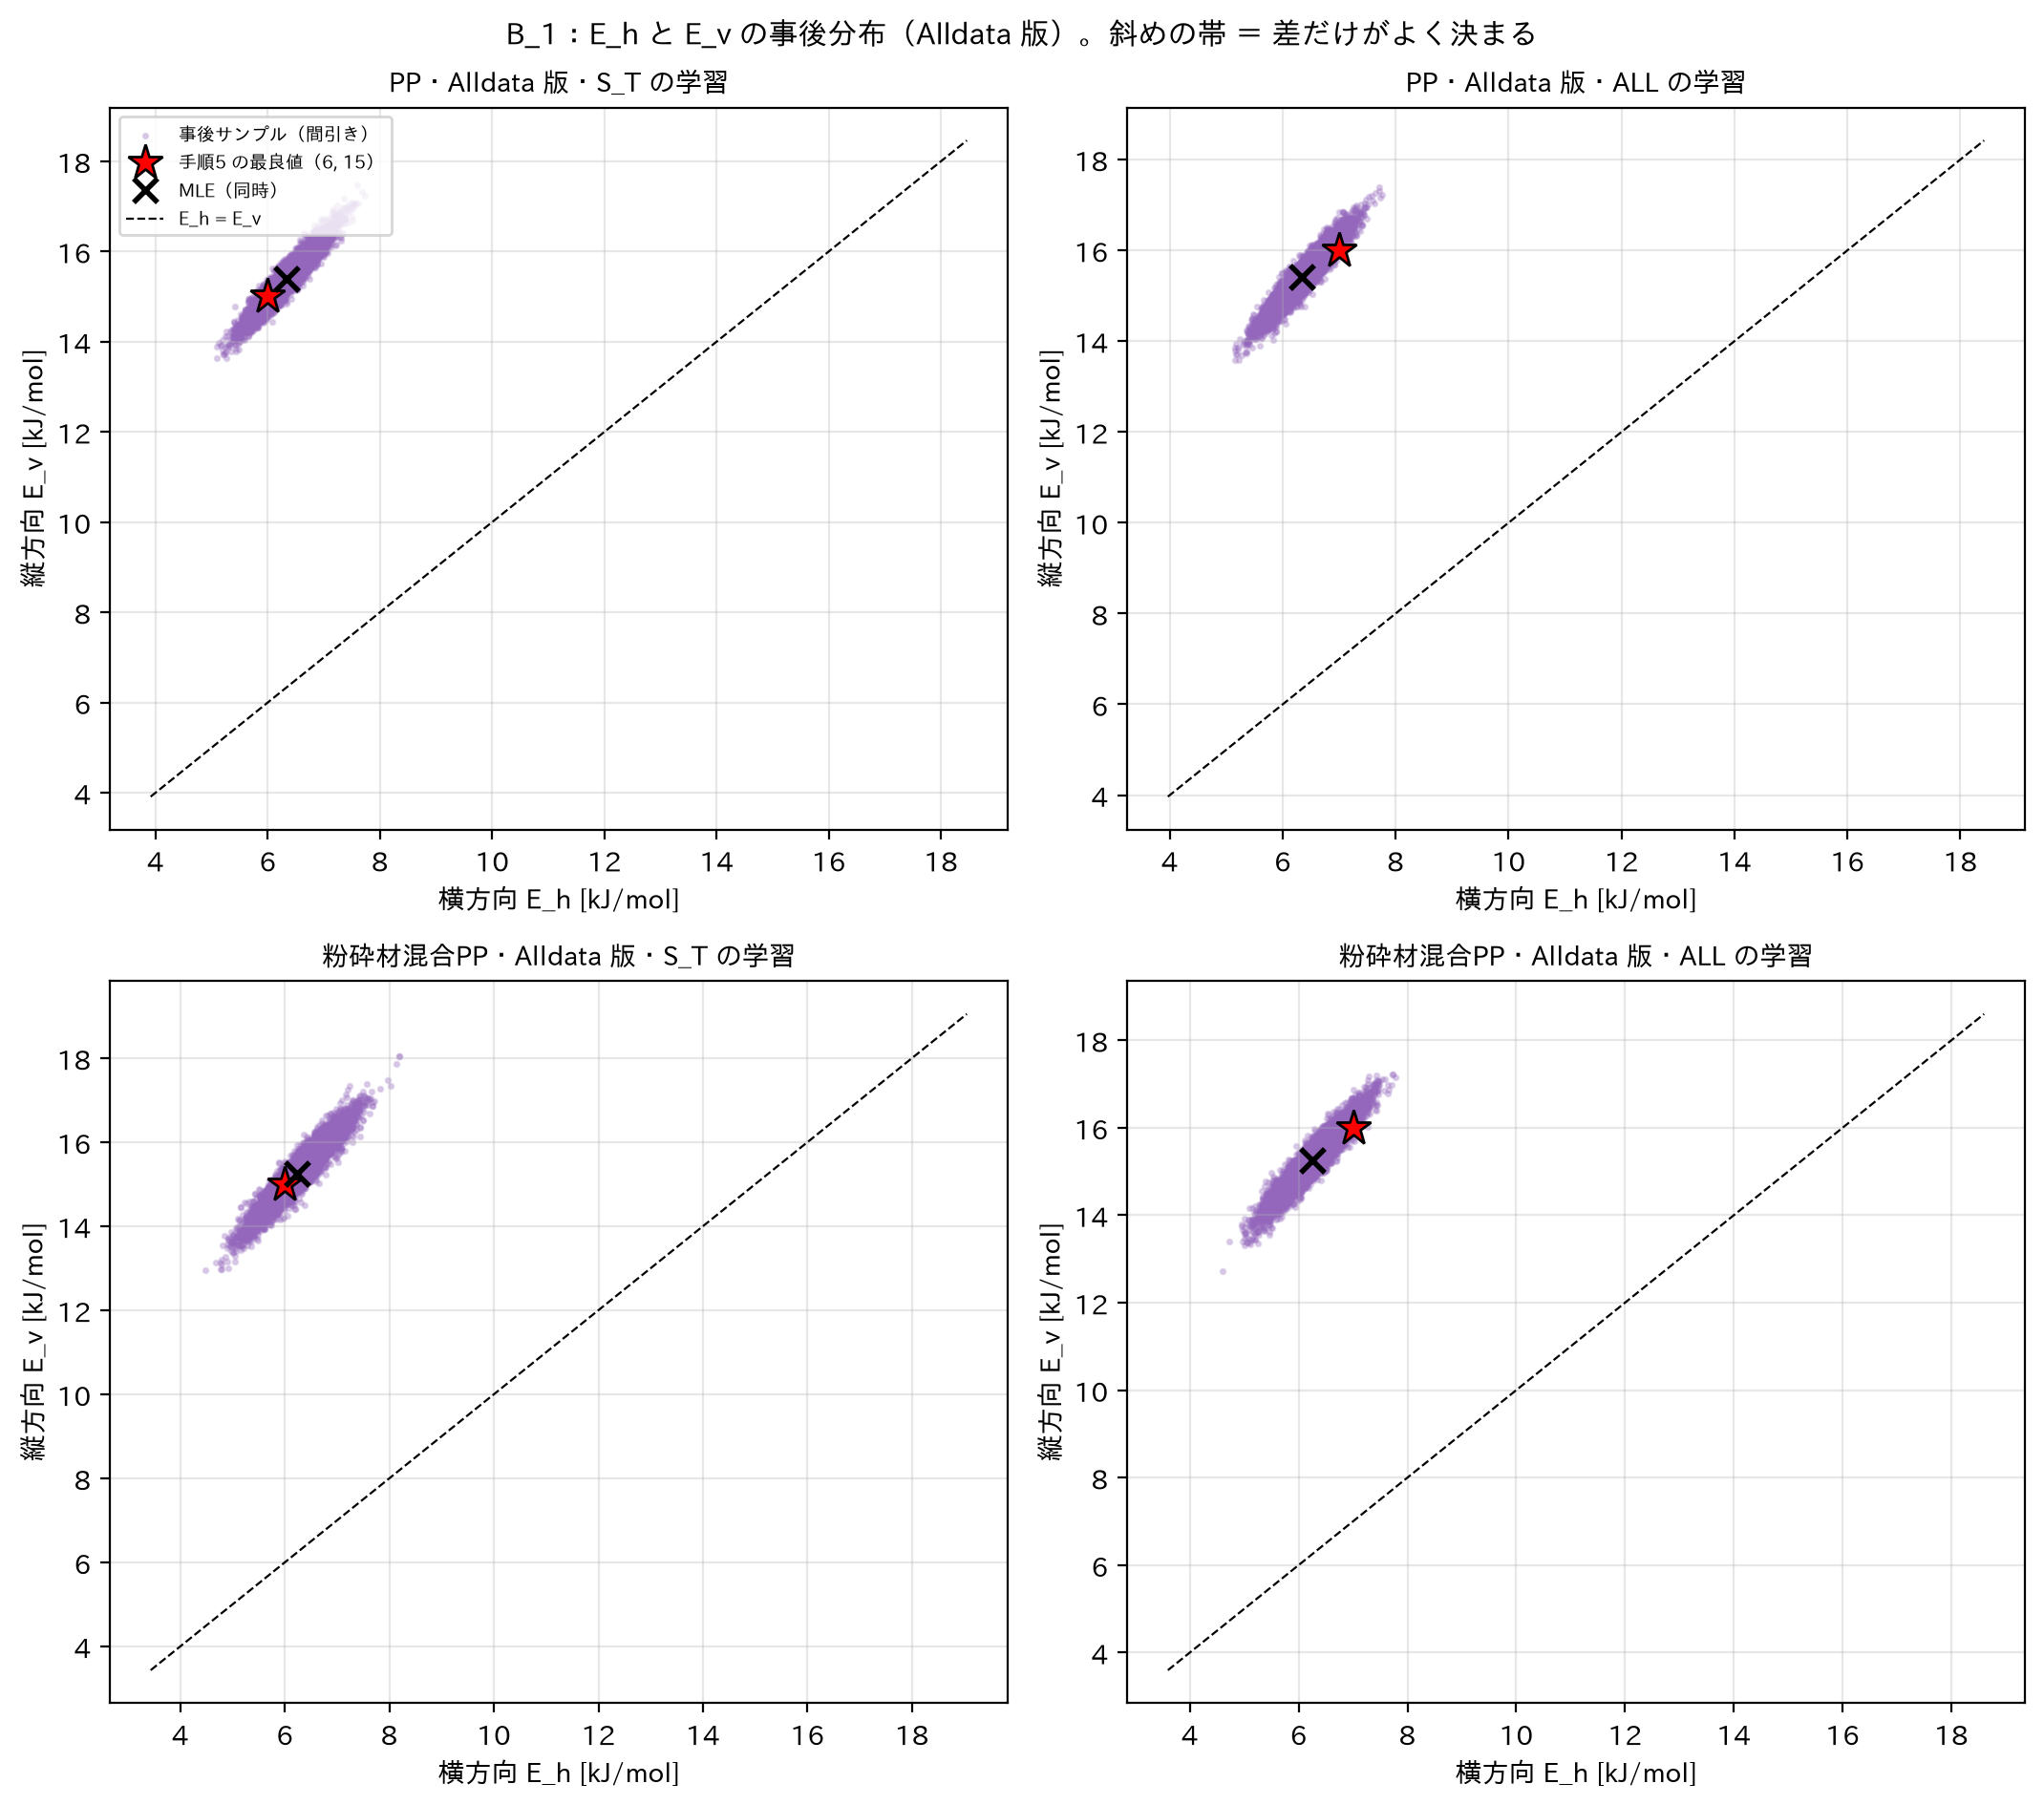
\includegraphics[width=0.85\linewidth]{fig1_E_posterior_Alldata.png}
\caption{B\_1 のずらし量の事後サンプル（上：PP、下：粉砕材混合 PP。左：S\_T の学習、右：ALL の学習）}
\end{figure}
\begin{points}
\pt{何を示す図か}B\_1 の温度のずらし量（横方向 $\Eh$、縦方向 $\Ev$）を、ハイパーパラメータと同時にサンプリングした結果です。1 つの点が 1 つのサンプルです。（ファイル：\file{fig1_E_posterior_Alldata.png}。\file{highres/} に 600 dpi 版もあります）
\pt{軸と記号}横軸が $\Eh$、縦軸が $\Ev$（kJ/mol）。紫の点が事後サンプル（間引き）、赤い星が手順5のプロファイル尤度の最良値、黒い $\times$ が MLE（同時）、破線が $\Eh=\Ev$（当初の構造 H）。
\pt{見るポイント}点が狭い範囲に集まっているか。細い斜めの帯（右上がり）になっていれば、「差 $\Ev-\Eh$ がよく決まる」ことを表す。星と $\times$ が、点の雲の中にあるか。
\pt{今回の結果}点は、右上がりの細い帯になりました（相関 0.95）。$\Eh$ は約 6〜7、$\Ev$ は約 15〜16 kJ/mol の狭い範囲で、破線（$\Eh=\Ev$）からは大きく離れています。星と $\times$ は、どちらも雲の中です。手順5のプロファイル尤度の最良値は、16 組すべてで、事後分布の 95\% 区間に入りました（表\ref{tab:E}）。
\end{points}

\subsection{図2：差 $\Ev-\Eh$ の事後分布（Alldata 版）}
\begin{figure}[H]
\centering
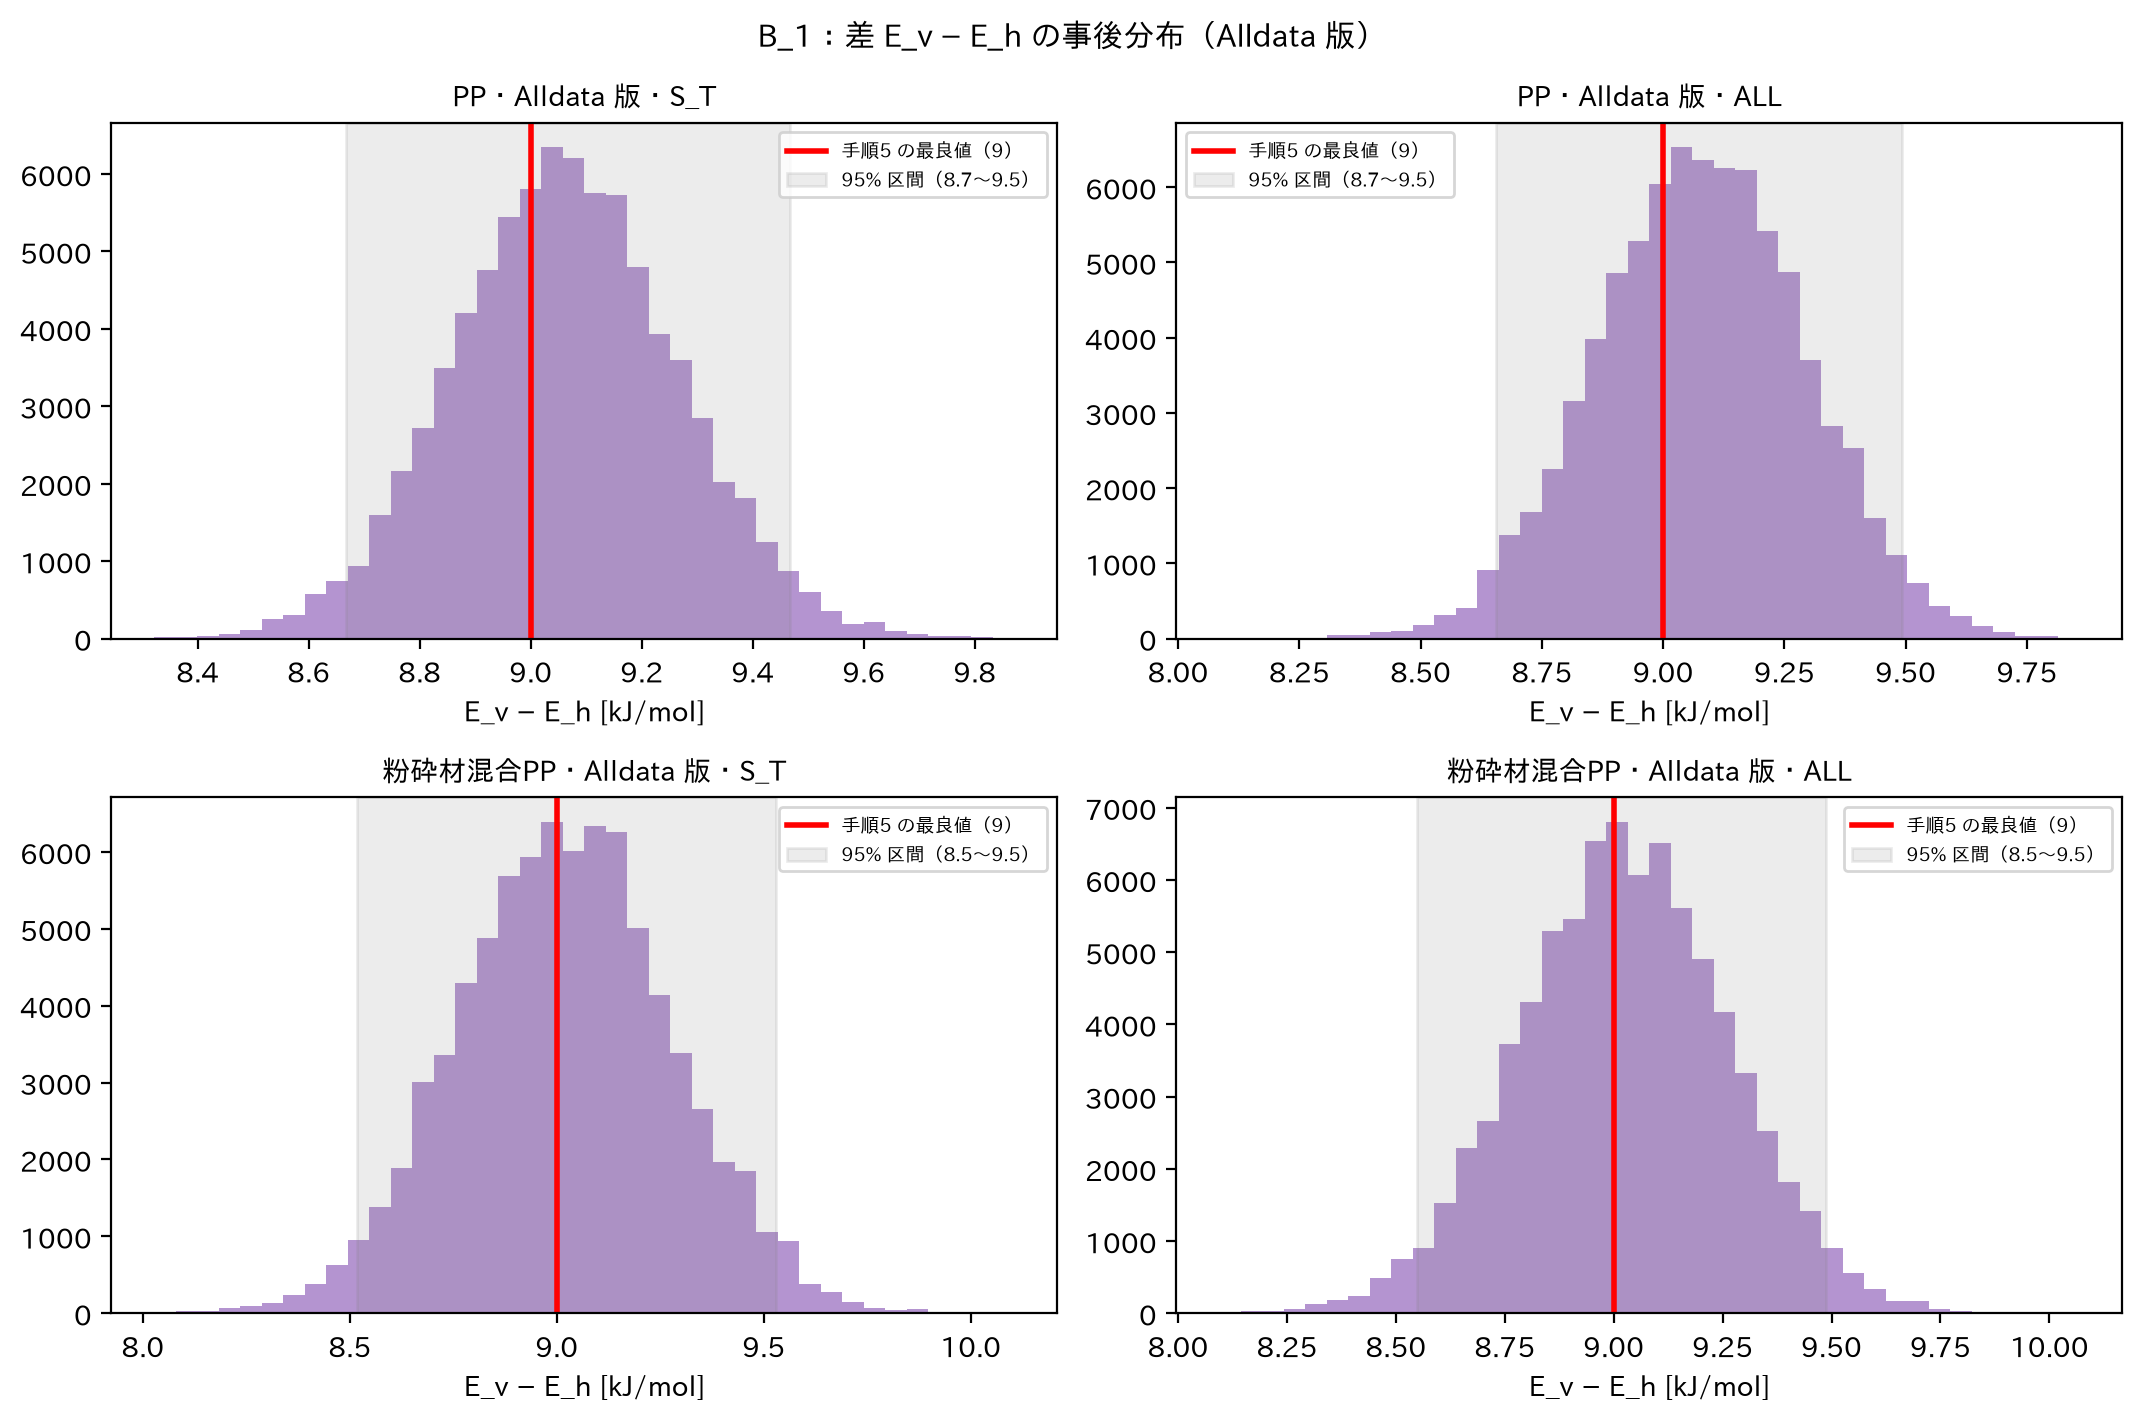
\includegraphics[width=0.8\linewidth]{fig2_E_diff_Alldata.png}
\caption{差 $\Ev-\Eh$ のヒストグラム（赤い線：手順5の最良値、灰色の帯：95\% 区間）}
\end{figure}
\begin{points}
\pt{何を示す図か}図1の斜めの帯の方向を、1 つの数にまとめた図です。（ファイル：\file{fig2_E_diff_Alldata.png}。\file{highres/} に 600 dpi 版もあります）
\pt{軸と記号}横軸が $\Ev-\Eh$（kJ/mol）、縦軸がサンプルの数。
\pt{見るポイント}山が細いか。赤い線が山の中にあるか。
\pt{今回の結果}差の標準偏差は 0.21 kJ/mol で、$\Eh$（0.37）や $\Ev$（0.53）の標準偏差より小さく、差が最もよく決まっています。PP の ALL で、差は 9.1（95\% 区間 8.7〜9.5）kJ/mol です。
\end{points}

\subsection{図3：ハイパーパラメータの事後分布（B\_1、PP・Alldata 版・ALL）}
\begin{figure}[H]
\centering
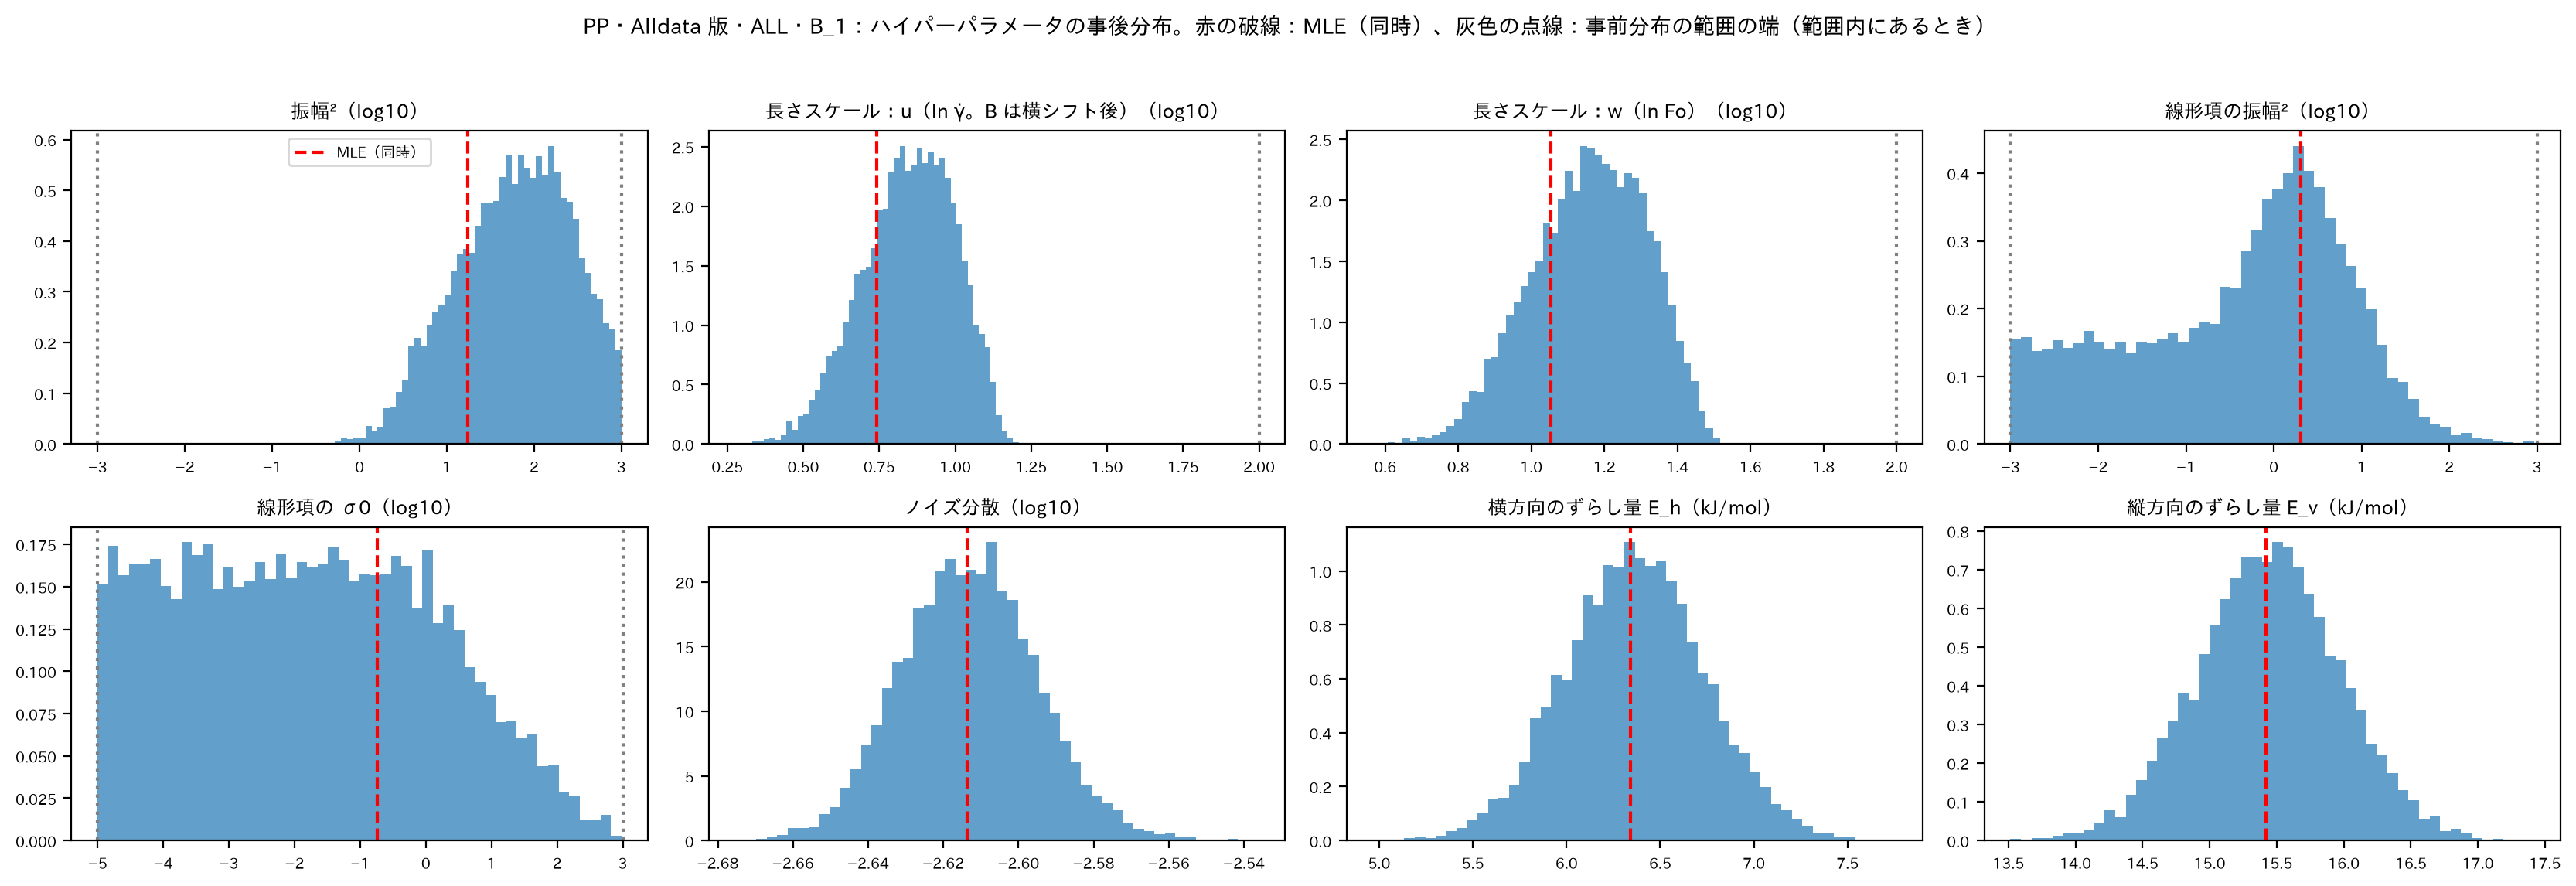
\includegraphics[width=1.0\linewidth]{fig3_posterior_Alldata_PP_B_1.png}
\caption{B\_1 のハイパーパラメータとずらし量の事後分布（赤の破線：MLE（同時）、灰色の点線：事前分布の範囲の端）}
\end{figure}
\begin{points}
\pt{何を示す図か}各ハイパーパラメータが、データでどれくらい決まっているかを示した図です。1 枚が 1 つのモデルです。（ファイル：\file{fig3_posterior_Alldata_PP_B_1.png}。\file{highres/} に 600 dpi 版もあります）
\pt{軸と記号}横軸は値（ずらし量は kJ/mol、それ以外は常用対数）、縦軸は密度。赤い破線が最尤推定値、灰色の点線が事前分布の範囲の端（範囲内にあるとき）。
\pt{見るポイント}山が細いほど、データでよく決まっている。山が範囲の端まで広がっていれば、データだけでは決まらない。赤い破線が山の中にあるか。
\pt{今回の結果}ノイズ分散は、95\% 区間の幅が中央値の約 16\% と、よく決まっています。$\Eh$・$\Ev$ も狭い山です。一方、関数の大きさ（振幅）は 95\% 区間の上限が下限の約 16 倍、線形項の $\sigma_0$ は $10^{-5}$ 付近から $10^{1.8}$ 付近まで、ほぼ平らに広がり、データでは決まりません。最尤推定は、これらの 1 点を選んでいただけで、その周りにほかの値も同じくらい許されることが分かります。
\end{points}

\subsection{図4：ハイパーパラメータの事後分布（C\_1、PP・5data 版・S\_V）}
\begin{figure}[H]
\centering
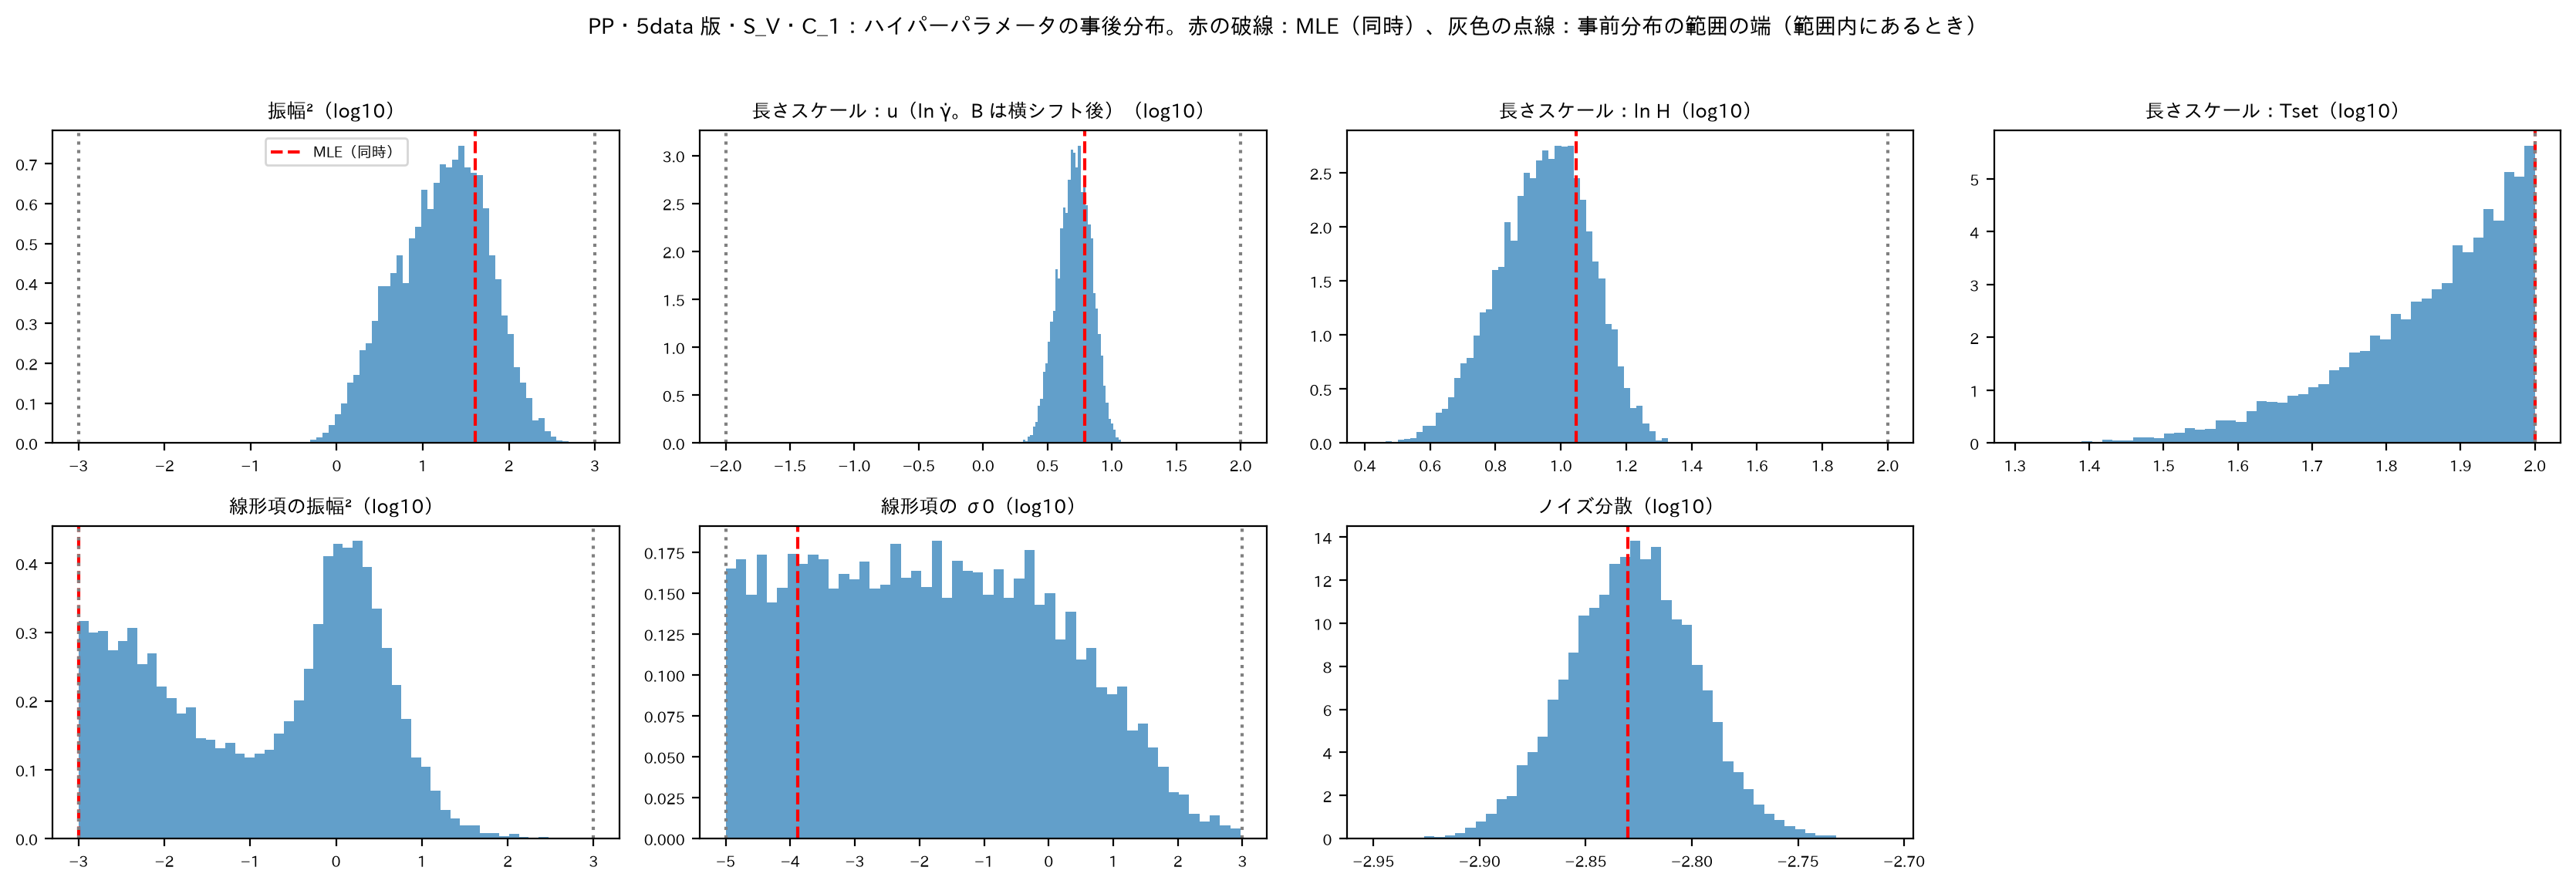
\includegraphics[width=1.0\linewidth]{fig3_posterior_5data_PP_C_1.png}
\caption{C\_1 のハイパーパラメータの事後分布}
\end{figure}
\begin{points}
\pt{何を示す図か}構造なしの C\_1 について、同じ種類の図を描いたものです。（ファイル：\file{fig3_posterior_5data_PP_C_1.png}。\file{highres/} に 600 dpi 版もあります）
\pt{軸と記号}図3と同じ。
\pt{見るポイント}$\Tset$ の長さスケールが、上限（灰色の点線）に張り付いていないか。
\pt{今回の結果}$\Tset$ の長さスケールの山は、上限の 100 に届き（8 組すべて）、「$\Tset$ に対しては、ほぼ直線」であることを表します。温度の効果は、ほぼ線形項が担っています。線形項の振幅の二乗は、下限（$10^{-3}$）近くの山と、$10^{0}$ 付近の山の 2 つに分かれます。ノートの判定は、この点で ★ になります。
\end{points}

\subsection{図5：トレース（B\_1、PP・Alldata 版・ALL）}
\begin{figure}[H]
\centering
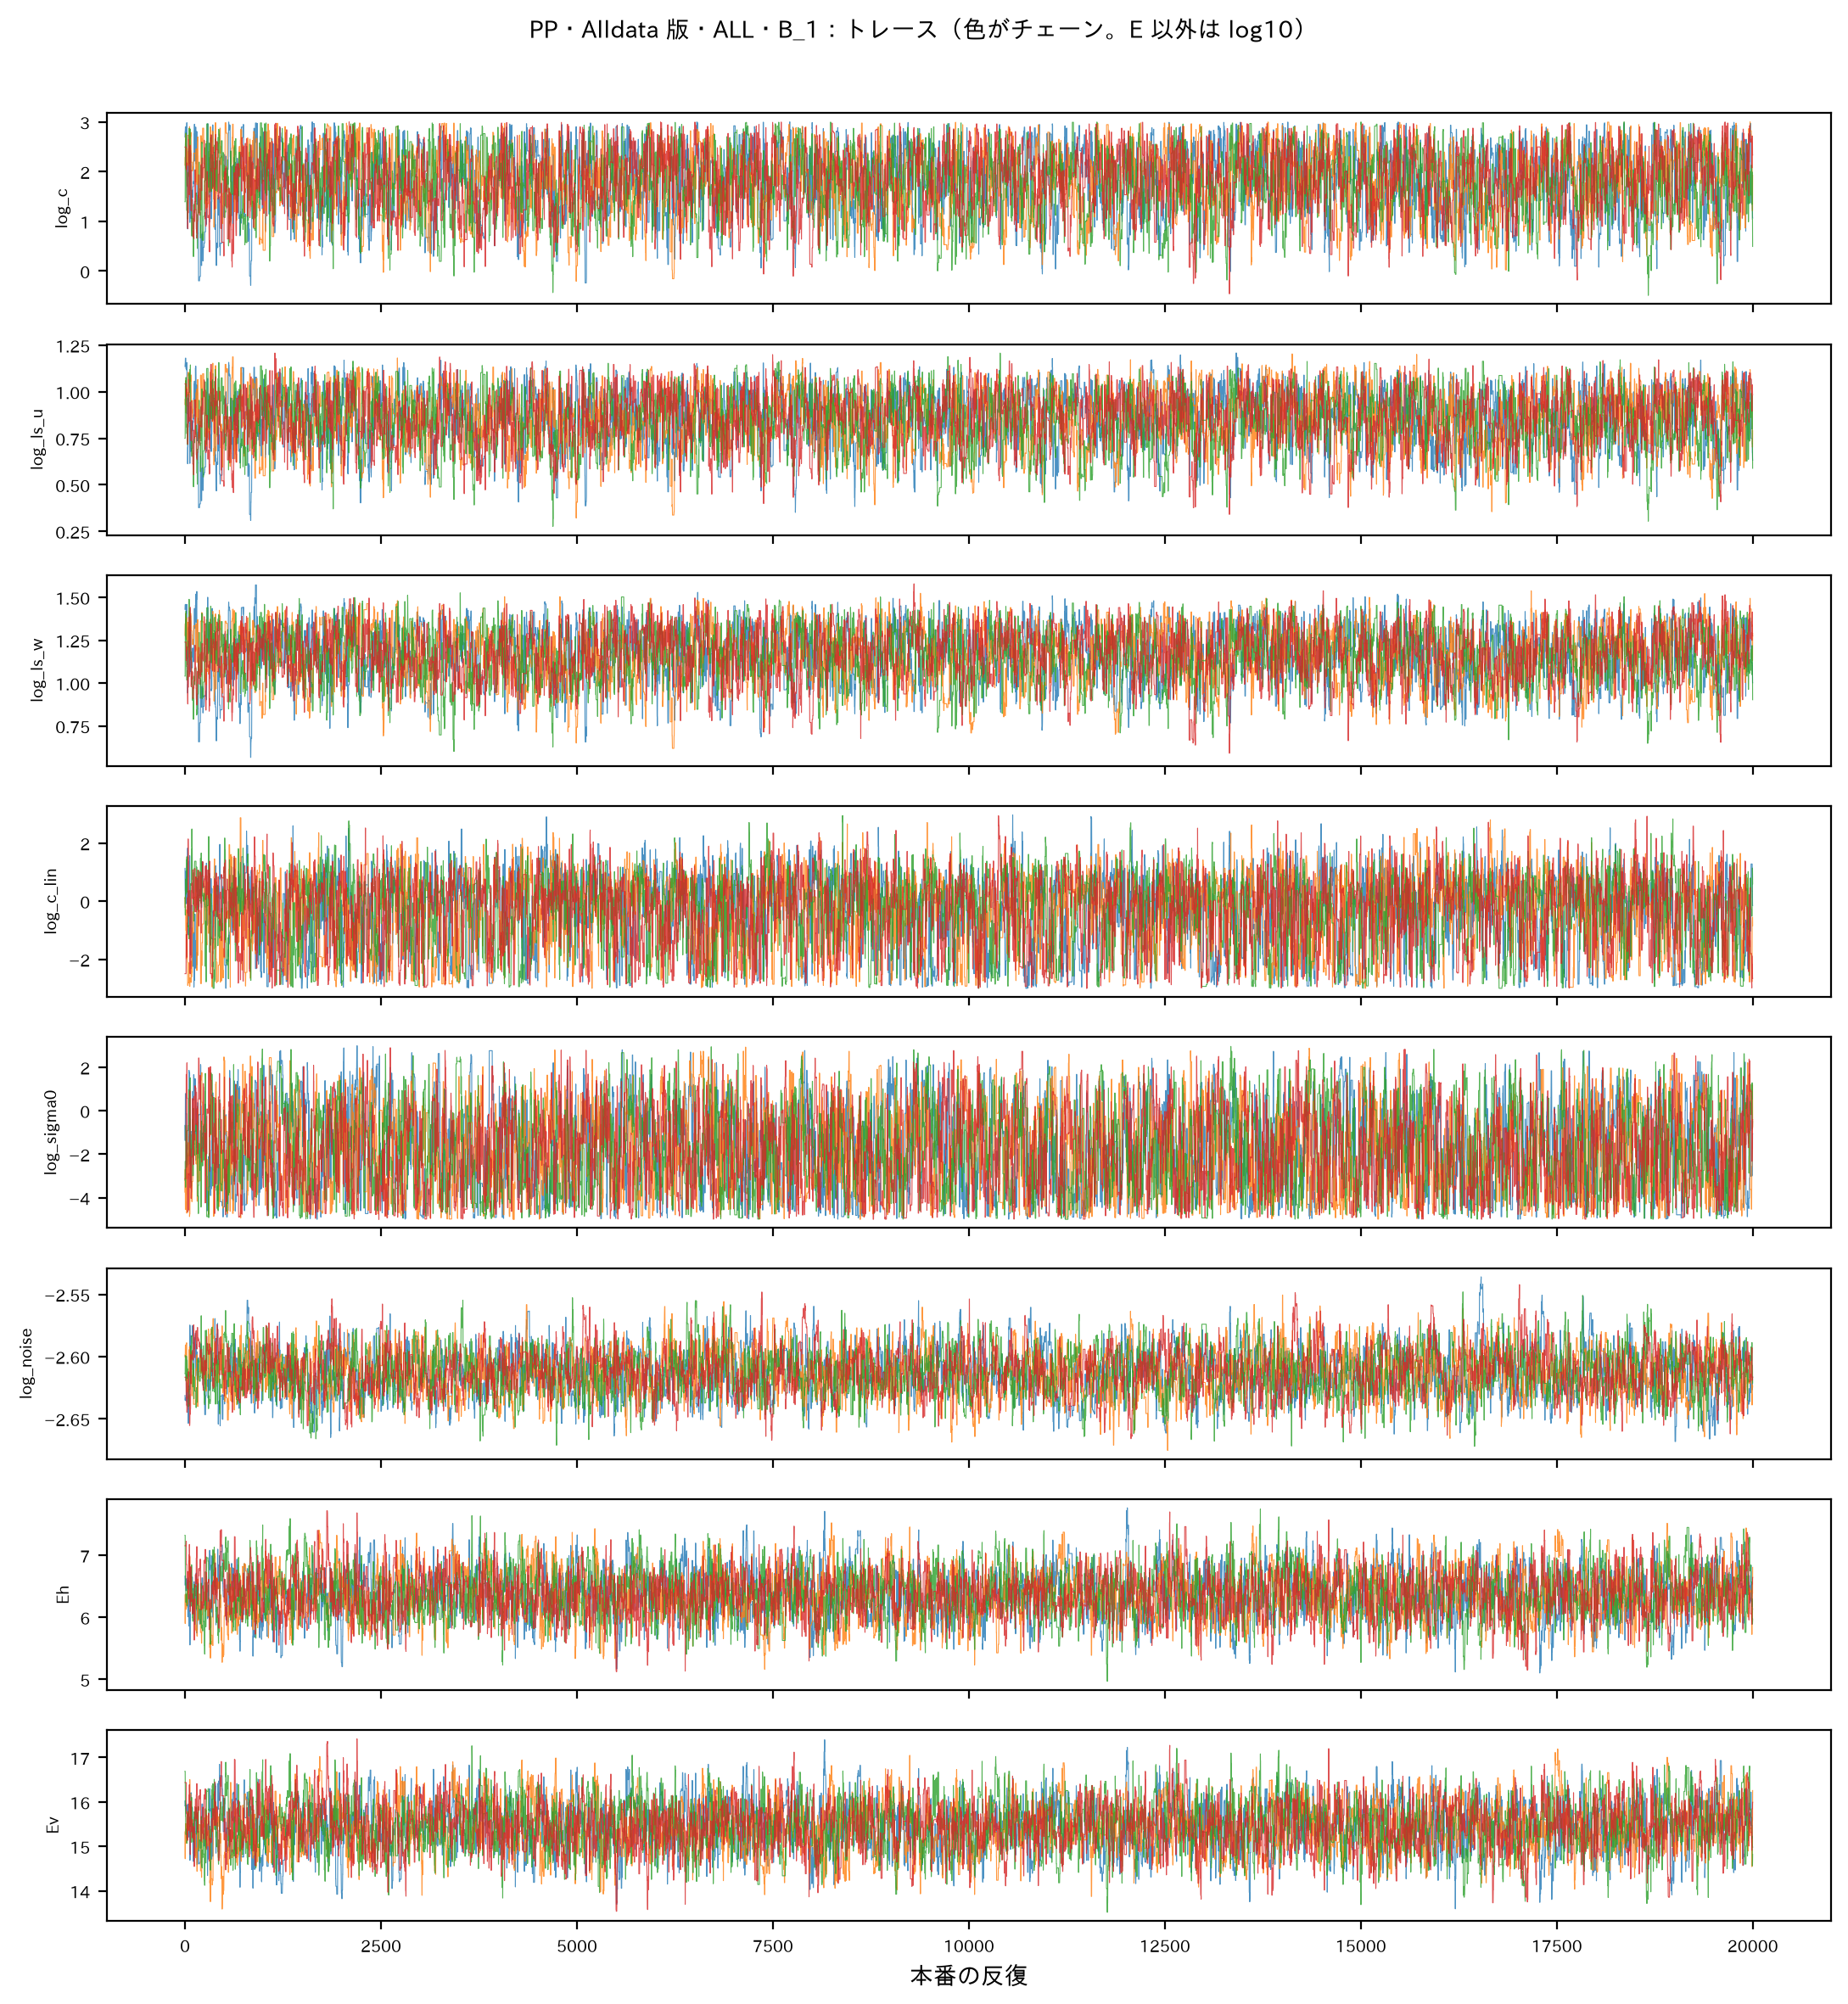
\includegraphics[width=0.95\linewidth]{fig4_trace_Alldata_PP_B_1.png}
\caption{サンプルの推移（色が 4 本のチェーン。ずらし量以外は常用対数）}
\end{figure}
\begin{points}
\pt{何を示す図か}サンプルが、きちんと混ざっているかを確かめる図です（収束診断の目で見る版）。（ファイル：\file{fig4_trace_Alldata_PP_B_1.png}。\file{highres/} に 600 dpi 版もあります）
\pt{軸と記号}横軸が本番の反復の順番、縦軸が値。色がチェーン。
\pt{見るポイント}4 色が、同じ範囲を重なって行き来していれば（毛虫のように）、収束しています。特定の色だけが別の所にいる、一方向にずっと動いている、は問題のしるし。
\pt{今回の結果}4 本のチェーンは、どのパラメータでも同じ範囲を重なって行き来しています。数値でも、R-hat は最大 1.008、ESS（bulk）は最小 1303 で、基準（1.01 以下、400 以上）を満たしました（表\ref{tab:conv}）。
\end{points}

\subsection{図6：予測指標の比較（5data 版）}
\begin{figure}[H]
\centering
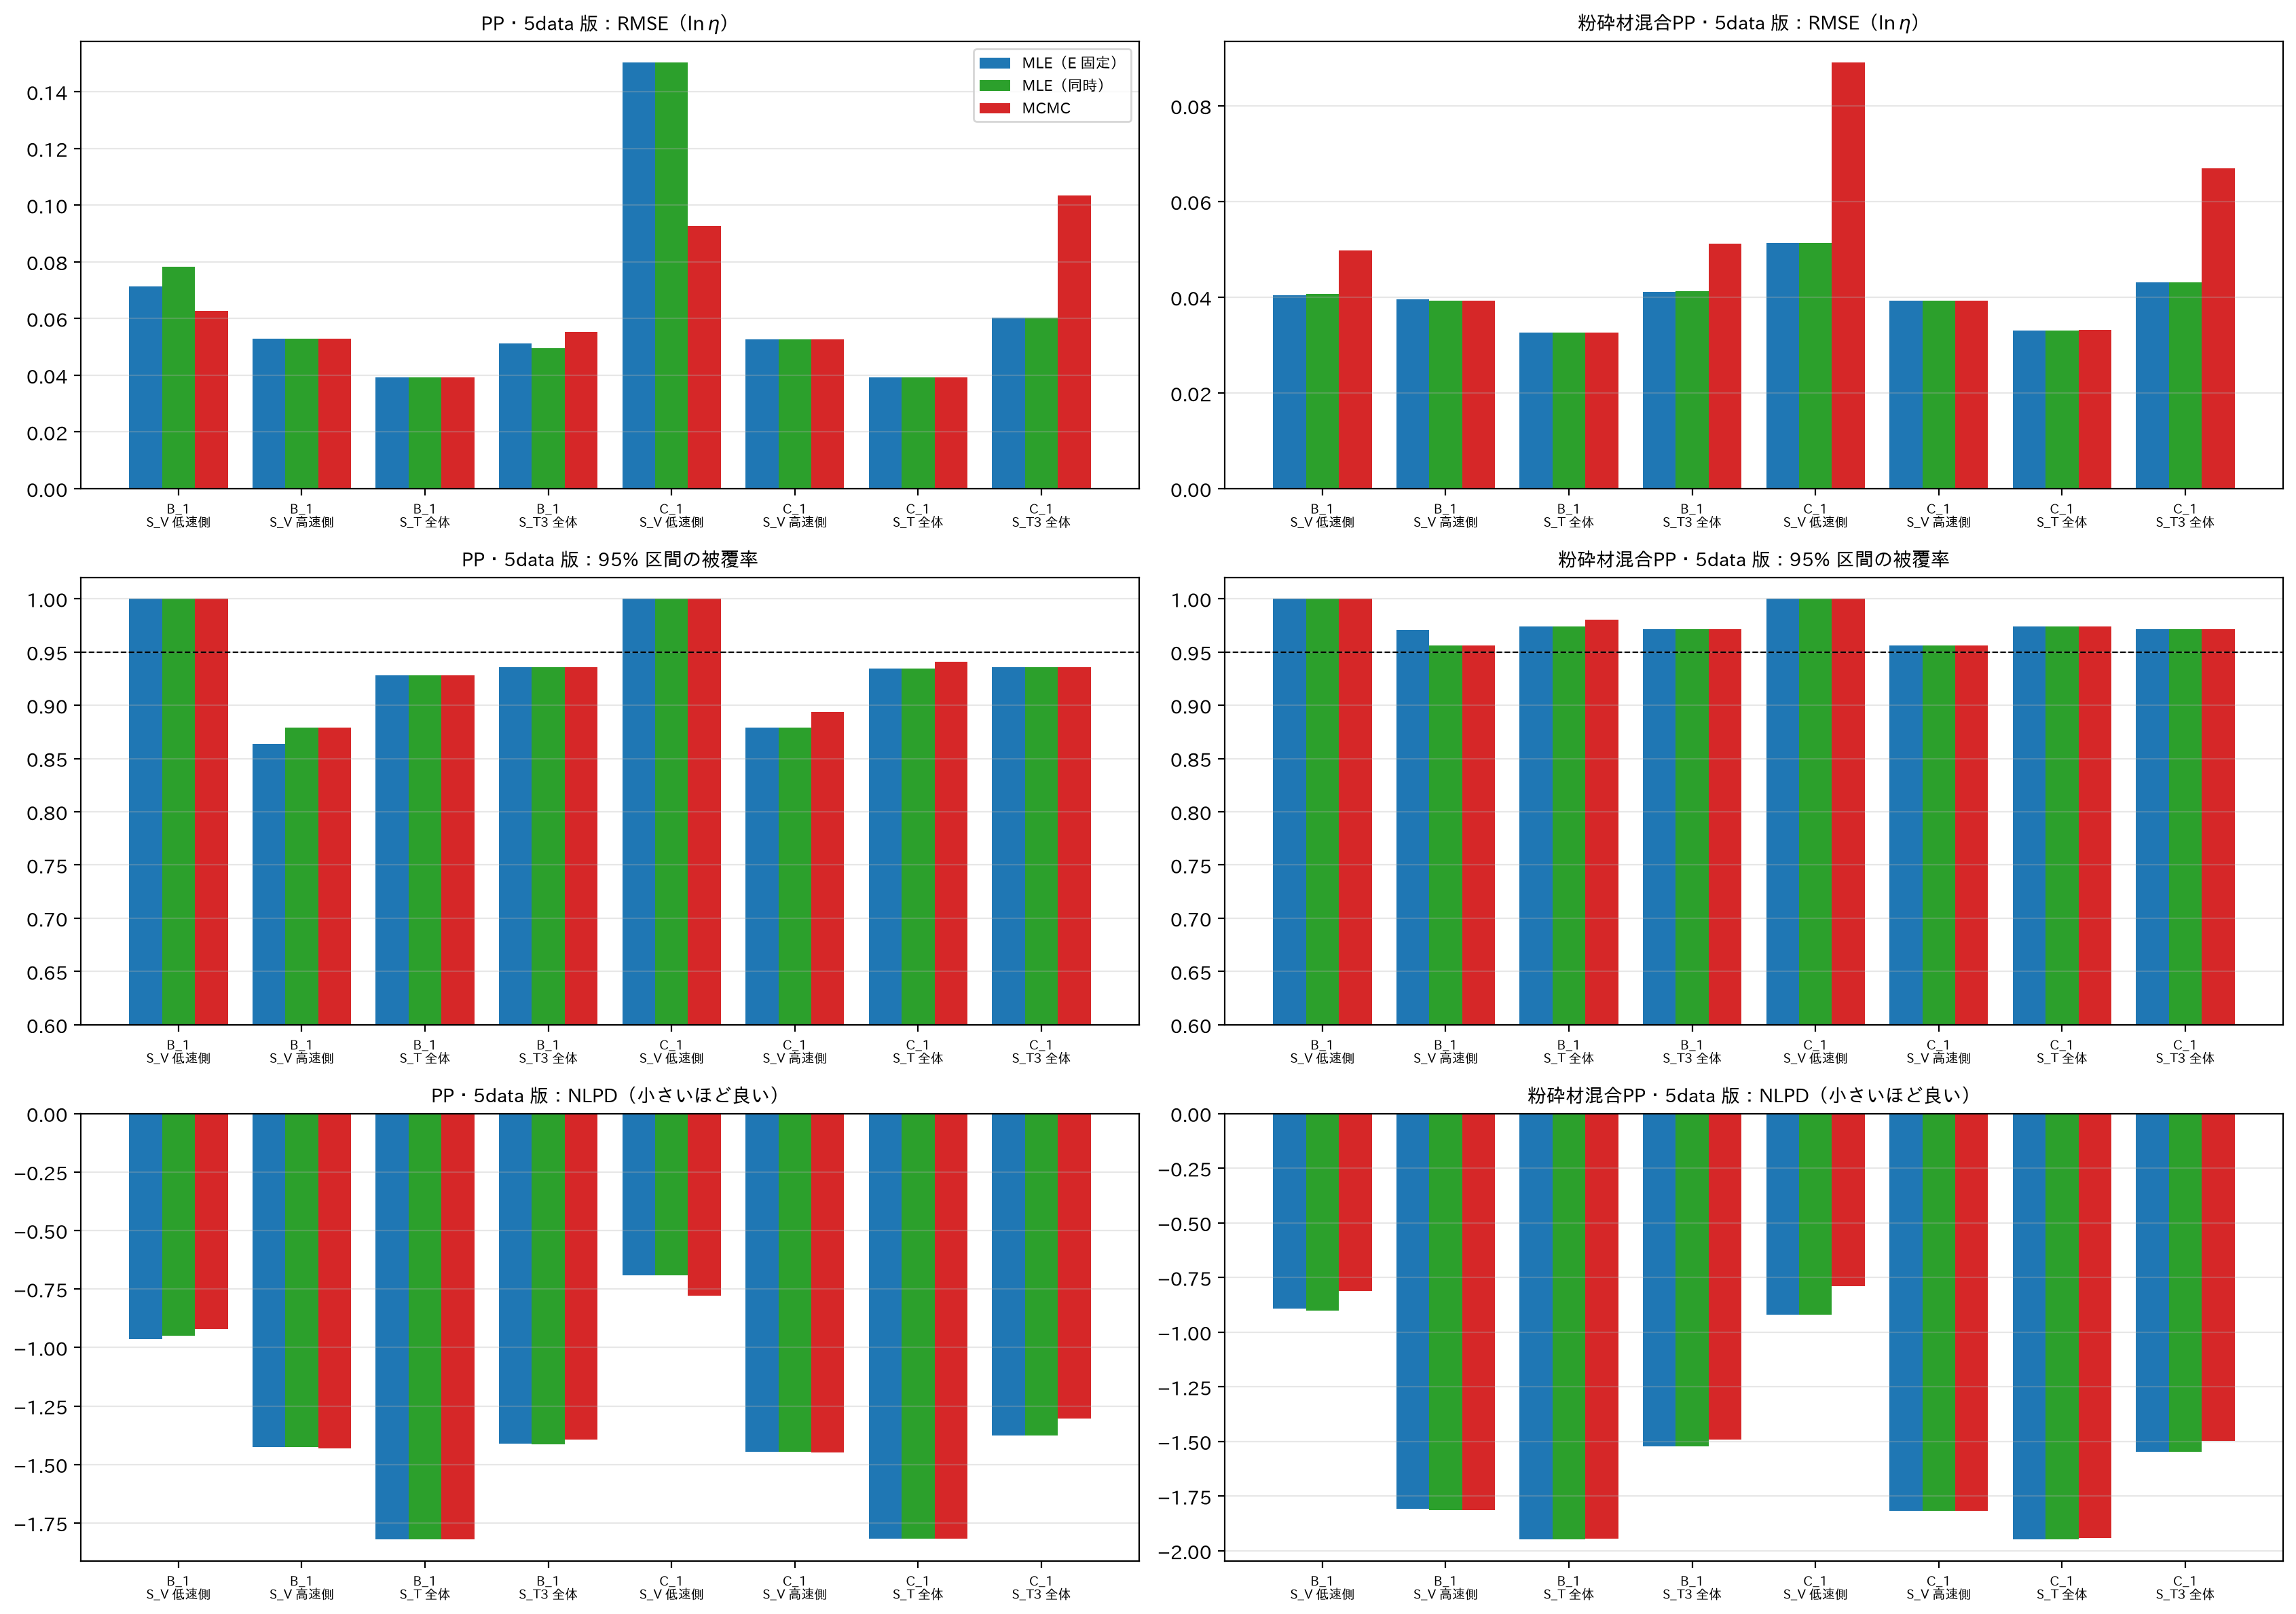
\includegraphics[width=1.0\linewidth]{fig5_metrics_5data.png}
\caption{最尤推定と MCMC の RMSE・被覆率・NLPD（左：PP、右：粉砕材混合 PP。色が方法）}
\end{figure}
\begin{points}
\pt{何を示す図か}3 通りの方法（MLE（E 固定）、MLE（同時）、MCMC）の予測を、モデルと検証の種類ごとに並べた図です。（ファイル：\file{fig5_metrics_5data.png}。\file{highres/} に 600 dpi 版もあります）
\pt{軸と記号}横軸がモデルと検証の種類。縦軸は上から、RMSE（小さいほどよい）、95\% 区間の被覆率（0.95 が理想）、NLPD（小さいほどよい）。
\pt{見るポイント}3 色の高さが同じなら、不確かさを取り込んでも、予測は変わらない。MCMC だけ高い（悪い）検証は、どれか。
\pt{今回の結果}S\_T（210 ℃）は、3 色ともほぼ同じです（PP の B\_1：0.039 と 0.039）。学習の範囲の外（S\_V の低速側、S\_T3）では、差が出ます。特に C\_1 は、最尤推定と MCMC の差が大きく、向きも一定しません（PP の S\_T3：0.060 から 0.103 へ悪化、PP の S\_V：0.092 から 0.067 へ改善）。B\_1 の動きは小さい（PP の S\_T3：0.051 から 0.055、S\_V：0.059 から 0.056）。表\ref{tab:met_5data_PP}。
\end{points}

\subsection{図7：設定温度の効果の不確かさ（Alldata 版）}
\begin{figure}[H]
\centering
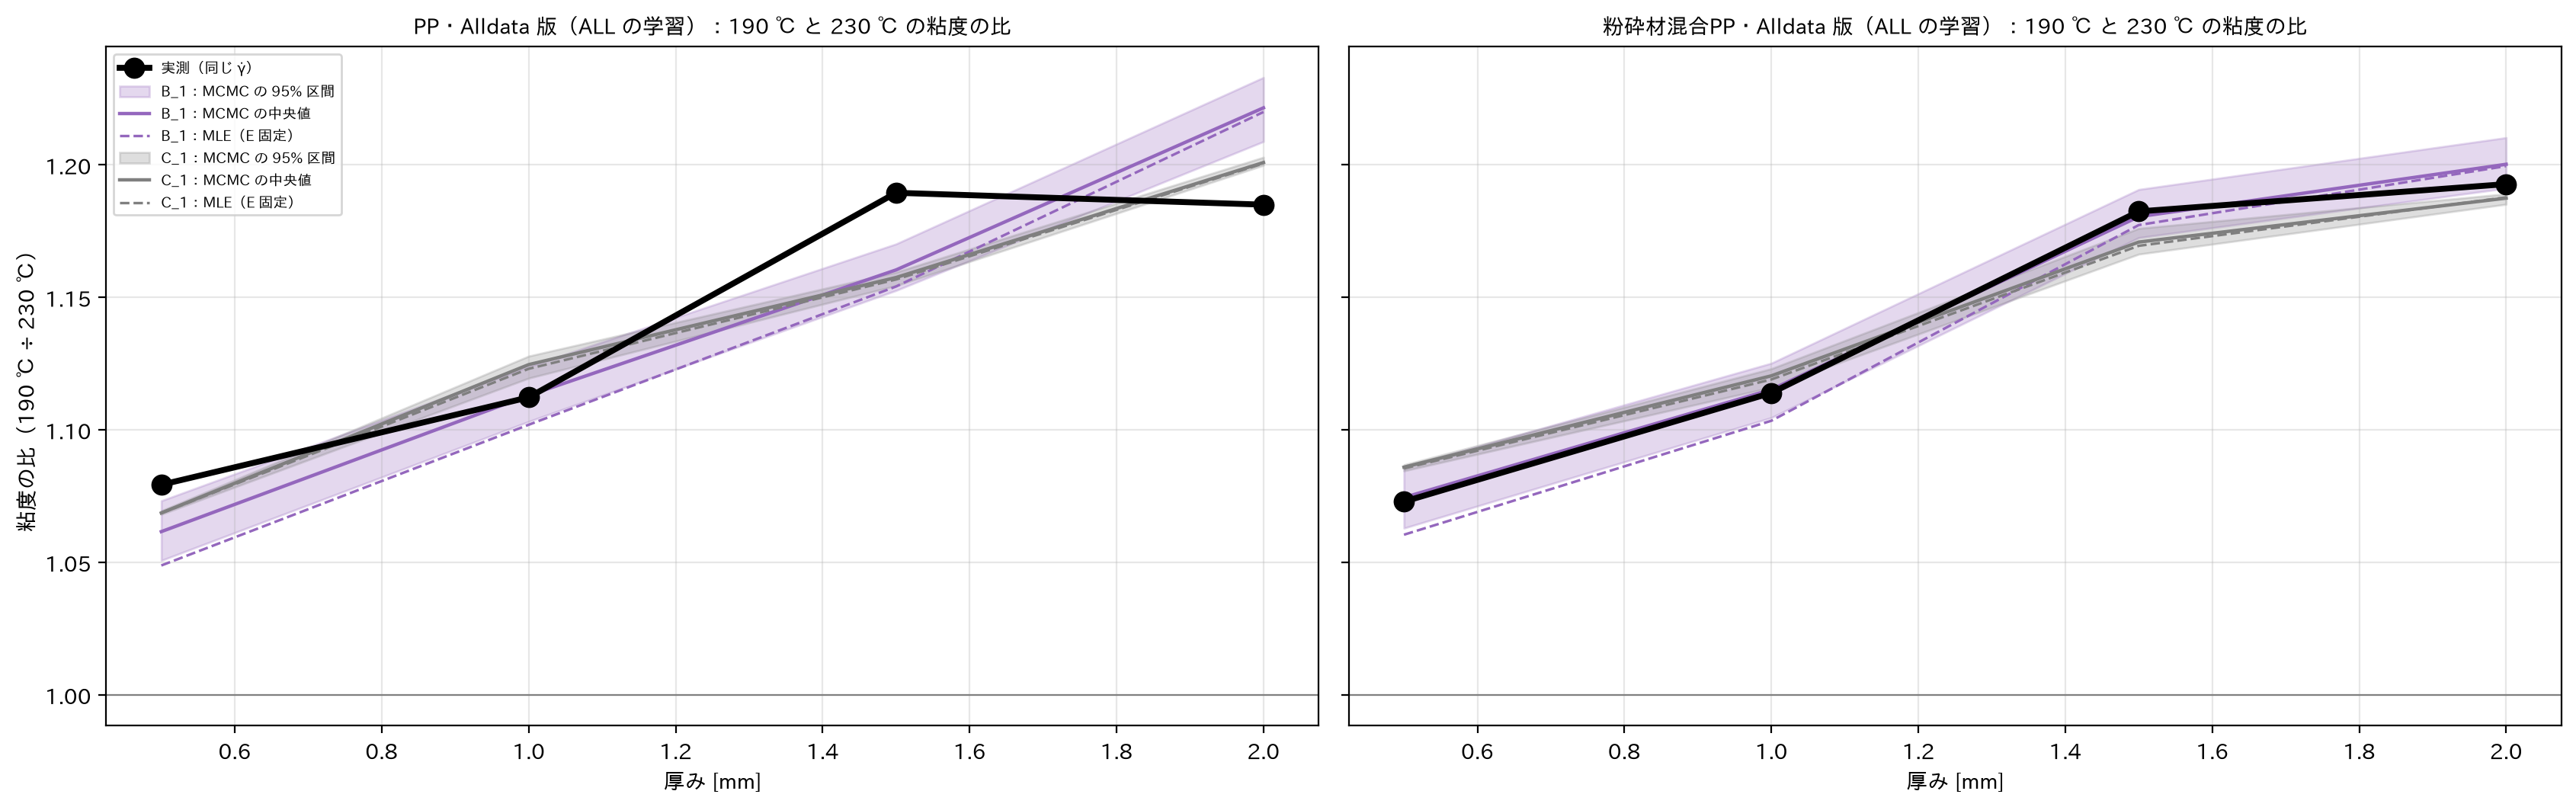
\includegraphics[width=1.0\linewidth]{fig6_tset_effect_Alldata.png}
\caption{190 ℃ と 230 ℃ の粘度の比（太い黒線：実測、帯：MCMC の 95\% 区間、破線：MLE（E 固定））}
\end{figure}
\begin{points}
\pt{何を示す図か}Tset だけを 190 ℃ から 230 ℃ に変えたときの粘度の比を、厚みごとに、実測と比べた図です。帯の幅が、ハイパーパラメータとずらし量の不確かさによる、予測の平均の不確かさです。（ファイル：\file{fig6_tset_effect_Alldata.png}。\file{highres/} に 600 dpi 版もあります）
\pt{軸と記号}横軸は厚み [mm]、縦軸は粘度の比。紫が B\_1、灰色が C\_1。
\pt{見るポイント}実測が帯の中に入っているか。帯が広いか狭いか。
\pt{今回の結果}B\_1 の帯は、厚いほど広がり（2.0 mm で約 $\pm$0.01）、C\_1 の帯は、ほぼ線のように狭くなります（C\_1 は温度の効果を線形項で担うため、不確かさが小さく出ます）。粉砕材混合 PP では、実測が B\_1 の帯に 4 つの厚みすべてで入ります。PP では、実測の 1.5 mm の比（1.189）が、2.0 mm（1.185）より大きく、モデルの滑らかな増加では表せないので、帯から外れる厚みがあります（表\ref{tab:tset}）。帯は、実測のばらつき（1 つの条件の比の誤差）ではなく、モデルの平均の不確かさだけです。
\end{points}

\subsection{図8：設定温度ごとの予測曲線（PP・5data 版、MCMC の混合分布）}
\begin{figure}[H]
\centering
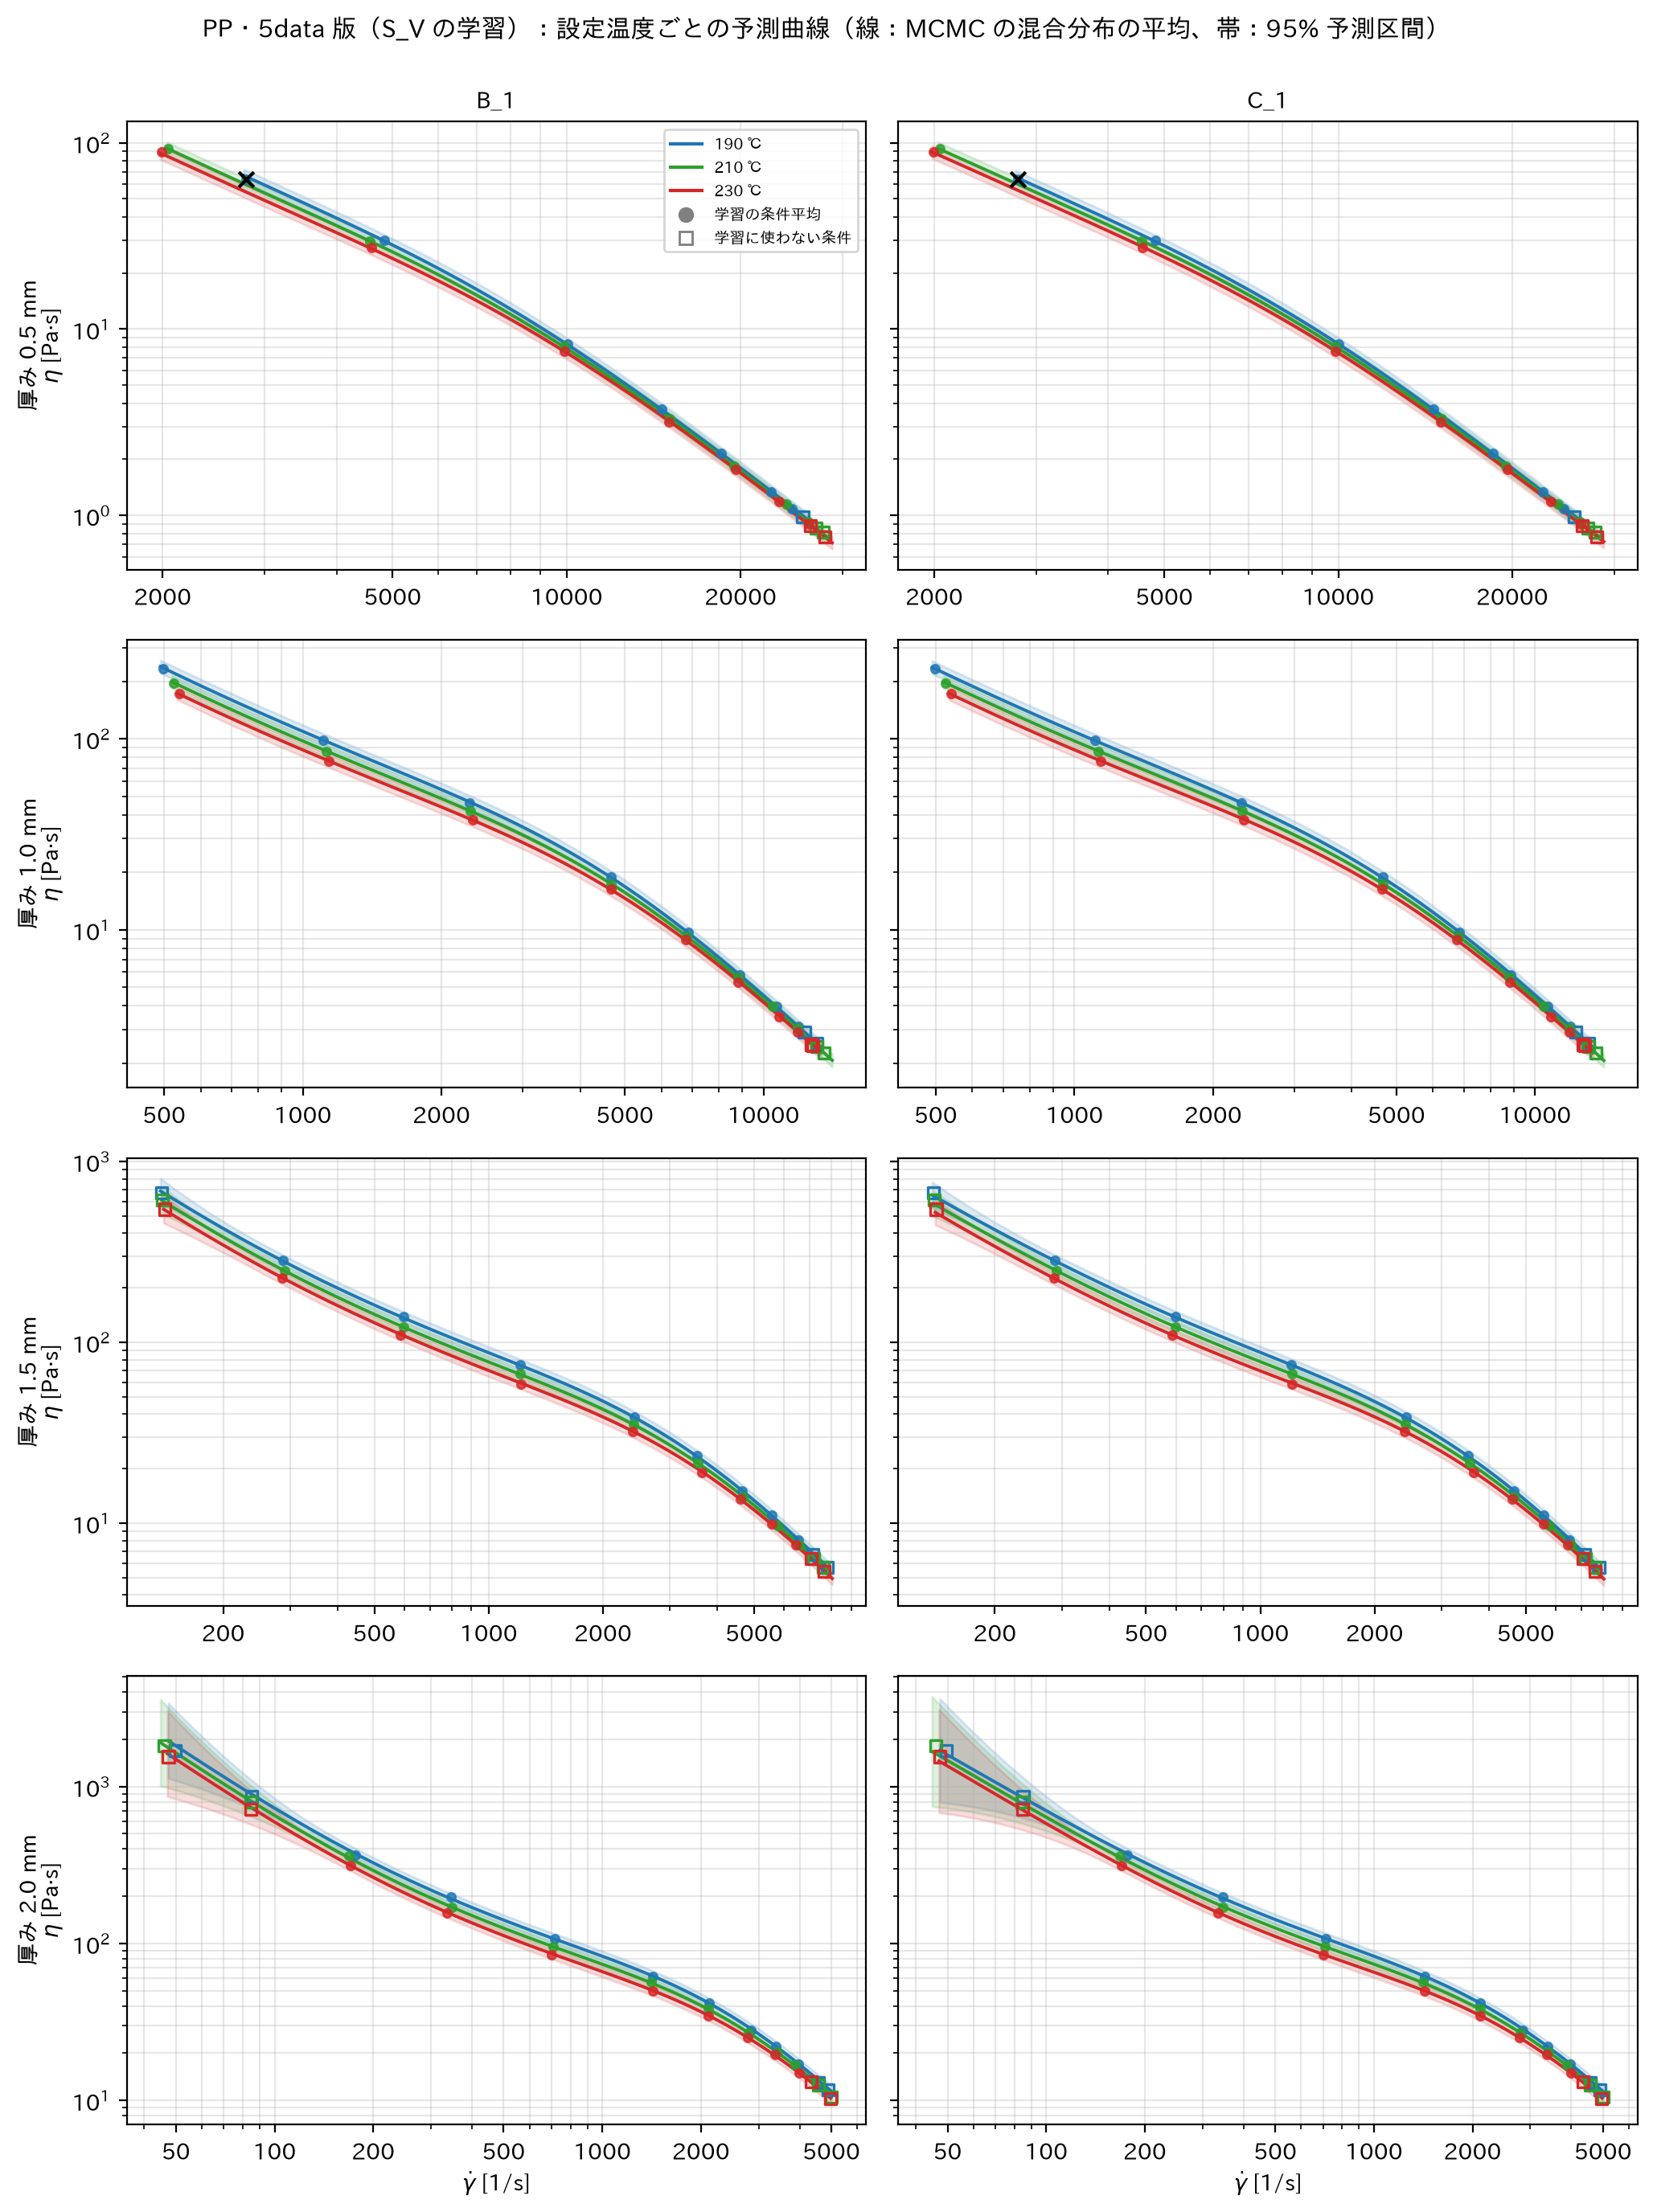
\includegraphics[width=0.85\linewidth]{fig7_curves_5data_PP.png}
\caption{MCMC の混合分布の予測平均と 95\% 予測区間（行が厚み、列が B\_1・C\_1）}
\end{figure}
\begin{points}
\pt{何を示す図か}不確かさを含めた最終的な予測を、せん断速度と粘度の関係として描いた図です。（ファイル：\file{fig7_curves_5data_PP.png}。\file{highres/} に 600 dpi 版もあります）
\pt{軸と記号}横軸はせん断速度、縦軸は粘度（どちらも対数）。青 190 ℃・緑 210 ℃・赤 230 ℃。点が学習の条件平均、白抜きの四角が学習に使わない条件（検証）、$\times$ は感度確認の条件。
\pt{見るポイント}点が帯の中に入っているか。学習の範囲の外で、帯が広がっているか。
\pt{今回の結果}B\_1 と C\_1 は、学習の範囲の中では、ほとんど同じ曲線と帯です。学習の範囲の外（2.0 mm の低せん断速度側）では、帯が大きく広がり、白抜きの検証の点が帯の中に入ります。
\end{points}


% =====================================================================
\section{表の見方}


\subsection{表\ref{tab:conv}：収束診断}
\begin{table}[H]
\caption{収束診断（学習データごとの最悪値。R-hat は最大、ESS(bulk) は最小、採択率は範囲）。右端は、事後分布の 95\% 区間が事前分布の範囲の端に届いたパラメータの数}\label{tab:conv}
\small
\begin{tabularx}{\linewidth}{@{}lllrrXr@{}}
\toprule
材料 & 版 & モデル & R-hat & ESS & 採択率 & 端 \\
\midrule
PP & 5data & B\_1 & 1.005 & 1942 & 0.20〜0.24 & 0 \\
 & 5data & C\_1 & 1.004 & 1554 & 0.20〜0.27 & 2 \\
 & Alldata & B\_1 & 1.004 & 2031 & 0.22〜0.25 & 0 \\
 & Alldata & C\_1 & 1.004 & 1387 & 0.22〜0.24 & 2 \\
粉砕材混合 PP & 5data & B\_1 & 1.003 & 1979 & 0.22〜0.27 & 0 \\
 & 5data & C\_1 & 1.005 & 1563 & 0.22〜0.25 & 2 \\
 & Alldata & B\_1 & 1.005 & 2106 & 0.22〜0.26 & 0 \\
 & Alldata & C\_1 & 1.008 & 1303 & 0.22〜0.27 & 2 \\
\bottomrule
\end{tabularx}
\end{table}
\begin{points}
\pt{読み方}R-hat は最大 1.008（目安 1.01 以下）、ESS は最小 1303（目安 400 以上）で、16 組すべてが収束しました。採択率は 0.20〜0.27（目標 0.234）。「端」の列は、C\_1 で、各学習データ 1 個ずつ（$\Tset$ の長さスケール）です。B\_1 は 0 です。
\end{points}

\subsection{表\ref{tab:E}：ずらし量の事後分布}
\begin{table}[H]
\caption{B\_1 のずらし量（kJ/mol）。事後の中央値（95\% 区間）。右端は、手順5のプロファイル尤度の最良値（$\Eh$・$\Ev$）}\label{tab:E}
\footnotesize
\begin{tabularx}{\linewidth}{@{}lllXXXl@{}}
\toprule
材料 & 版 & 学習 & $\Eh$ & $\Ev$ & $\Ev-\Eh$ & 手順5 \\
\midrule
PP & 5data & S\_V & 6.4（5.4〜7.4） & 15.7（14.3〜17.0） & 9.3（8.7〜9.8） & 6・15 \\
 & 5data & S\_T & 6.3（5.4〜7.2） & 15.5（14.3〜16.8） & 9.2（8.7〜9.7） & 6・15 \\
粉砕材混合 PP & 5data & S\_V & 6.3（5.4〜7.3） & 15.5（14.1〜16.8） & 9.1（8.6〜9.6） & 7・16 \\
 & 5data & S\_T & 6.3（5.3〜7.4） & 15.5（14.1〜16.9） & 9.1（8.6〜9.7） & 6・15 \\
PP & Alldata & S\_T & 6.3（5.6〜7.0） & 15.4（14.4〜16.4） & 9.1（8.7〜9.5） & 6・15 \\
 & Alldata & ALL & 6.4（5.6〜7.1） & 15.4（14.4〜16.5） & 9.1（8.7〜9.5） & 7・16 \\
粉砕材混合 PP & Alldata & S\_T & 6.3（5.3〜7.2） & 15.3（14.0〜16.5） & 9.0（8.5〜9.5） & 6・15 \\
 & Alldata & ALL & 6.3（5.4〜7.1） & 15.3（14.1〜16.5） & 9.0（8.5〜9.5） & 7・16 \\
\bottomrule
\end{tabularx}
\end{table}
\begin{points}
\pt{読み方}どの学習データでも、$\Eh$ は約 6.3、$\Ev$ は約 15.4 kJ/mol 前後で、95\% 区間の幅は、$\Eh$ で約 2、$\Ev$ で約 2.5 kJ/mol です。手順5の最良値（格子の値なので、整数）は、16 / 16 個が事後の 95\% 区間に入ります。同時最尤推定（約 6.3 と 15.4）は、事後の中央値と一致します。
\end{points}

\subsection{表\ref{tab:hp}：ハイパーパラメータの事後分布（Alldata 版・ALL）}
\begin{table}[H]
\caption{ハイパーパラメータとずらし量の、最尤推定（同時）と事後分布（中央値と 95\% 区間）。振幅・線形項の振幅は $\sqrt{\text{振幅}^2}$ の値、長さスケールは標準化した入力に対する値。右端：95\% 区間が事前分布の範囲の端に届いたか}\label{tab:hp}
\scriptsize
\begin{tabularx}{\linewidth}{@{}llrrXl@{}}
\toprule
モデル & パラメータ & MLE（同時） & 事後の中央値 & 95\% 区間 & 端 \\
\midrule
PP・B\_1 & 振幅 & 4.16 & 8.1 & 1.71〜27.5 &  \\
 & 長さスケール $u$（$\ln\gd$） & 5.51 & 7.18 & 3.41〜12.7 &  \\
 & 長さスケール $w$（$\ln\mathrm{Fo}$） & 11.3 & 14.7 & 6.9〜26.8 &  \\
 & 線形項の振幅 & 1.43 & 0.875 & 0.0381〜6 &  \\
 & 線形項の $\sigma_0$ & 0.181 & 0.0131 & 1.46e-5〜65.7 &  \\
 & ノイズ分散 & 2.43e-3 & 2.44e-3 & 2.25e-3〜2.65e-3 &  \\
 & $\Eh$ & 6.34 & 6.36 & 5.63〜7.1 &  \\
 & $\Ev$ & 15.4 & 15.4 & 14.4〜16.5 &  \\
\midrule
PP・C\_1 & 振幅 & 2.74 & 4.18 & 1.22〜11.6 &  \\
 & 長さスケール $u$（$\ln\gd$） & 3.72 & 4.37 & 2.42〜7.26 &  \\
 & 長さスケール $\ln H$ & 7.84 & 9.24 & 4.83〜16 &  \\
 & 長さスケール $\Tset$ & 72.6 & 79.4 & 40.5〜99.2 & はい \\
 & 線形項の振幅 & 1.49 & 0.899 & 0.0352〜4.57 &  \\
 & 線形項の $\sigma_0$ & 2.09e-5 & 9.34e-3 & 1.36e-5〜58.7 &  \\
 & ノイズ分散 & 2.43e-3 & 2.43e-3 & 2.24e-3〜2.64e-3 &  \\
\midrule
粉砕材混合 PP・B\_1 & 振幅 & 4.85 & 8.51 & 1.93〜27 &  \\
 & 長さスケール $u$（$\ln\gd$） & 6.01 & 7.52 & 3.7〜13.1 &  \\
 & 長さスケール $w$（$\ln\mathrm{Fo}$） & 11.8 & 14.6 & 6.88〜26.1 &  \\
 & 線形項の振幅 & 1.27 & 0.618 & 0.0372〜5.47 &  \\
 & 線形項の $\sigma_0$ & 3.61e-3 & 0.0143 & 1.50e-5〜78.8 &  \\
 & ノイズ分散 & 1.47e-3 & 1.47e-3 & 1.31e-3〜1.67e-3 &  \\
 & $\Eh$ & 6.25 & 6.27 & 5.43〜7.12 &  \\
 & $\Ev$ & 15.3 & 15.3 & 14.1〜16.5 &  \\
\midrule
粉砕材混合 PP・C\_1 & 振幅 & 2.72 & 5.03 & 1.34〜13.1 &  \\
 & 長さスケール $u$（$\ln\gd$） & 3.91 & 4.92 & 2.65〜8.04 &  \\
 & 長さスケール $\ln H$ & 7.55 & 9.74 & 4.74〜16.7 &  \\
 & 長さスケール $\Tset$ & 64.2 & 78.3 & 38〜99 & はい \\
 & 線形項の振幅 & 1.38 & 0.323 & 0.034〜3.68 &  \\
 & 線形項の $\sigma_0$ & 2.33e-4 & 0.0164 & 1.40e-5〜98.3 &  \\
 & ノイズ分散 & 1.42e-3 & 1.43e-3 & 1.27e-3〜1.61e-3 &  \\

\bottomrule
\end{tabularx}
\end{table}
\begin{points}
\pt{読み方}ノイズ分散は、最尤推定と事後の中央値がほぼ一致し、幅も狭い（よく決まっている）。振幅と線形項の振幅は、95\% 区間の幅が 10 倍以上、$\sigma_0$ は 6 桁以上に広がり、最尤推定の値は、その広い範囲の中の 1 点にすぎません。C\_1 の $\Tset$ の長さスケールは、上限（100）に届いています。
\end{points}

\subsection{表\ref{tab:met_5data_PP} ほか：予測の比較}
\begin{points}
\pt{表の種類}5data 版と Alldata 版、PP と粉砕材混合 PP の 4 つの表です。行が、モデル（B\_1・C\_1）と方法（MLE（E 固定）、MLE（同時）、MCMC）、列が検証の種類です。5data 版の S\_V は外挿（学習していない低速側・高速側）、S\_T は 210 ℃ の全条件、S\_T3 は 3data の 210 ℃（速度の外挿も重なる）。Alldata 版は、S\_T と、その S\_T3。
\end{points}
\begin{table}[H]
\caption{PP・5data 版：RMSE（括弧：95\% 区間の被覆率）。最尤推定と MCMC の比較}\label{tab:met_5data_PP}
\small
\begin{tabularx}{\linewidth}{@{}llXXXX@{}}
\toprule
モデル & 方法 & S\_V 全体 & S\_V 低速側 & S\_T & S\_T3 \\
\midrule
B\_1 & MLE（E 固定） & 0.059（0.90） & 0.071（1.00） & 0.039（0.93） & 0.051（0.94） \\
 & MLE（同時） & 0.061（0.91） & 0.078（1.00） & 0.039（0.93） & 0.050（0.94） \\
 & MCMC & 0.056（0.91） & 0.063（1.00） & 0.039（0.93） & 0.055（0.94） \\
\midrule
C\_1 & MLE（E 固定） & 0.092（0.91） & 0.150（1.00） & 0.039（0.93） & 0.060（0.94） \\
 & MLE（同時） & 0.092（0.91） & 0.150（1.00） & 0.039（0.93） & 0.060（0.94） \\
 & MCMC & 0.067（0.92） & 0.093（1.00） & 0.039（0.94） & 0.103（0.94） \\

\bottomrule
\end{tabularx}
\end{table}

\begin{table}[H]
\caption{粉砕材混合 PP・5data 版：RMSE（括弧：95\% 区間の被覆率）。最尤推定と MCMC の比較}\label{tab:met_5data_MIX}
\small
\begin{tabularx}{\linewidth}{@{}llXXXX@{}}
\toprule
モデル & 方法 & S\_V 全体 & S\_V 低速側 & S\_T & S\_T3 \\
\midrule
B\_1 & MLE（E 固定） & 0.040（0.98） & 0.040（1.00） & 0.033（0.97） & 0.041（0.97） \\
 & MLE（同時） & 0.040（0.97） & 0.041（1.00） & 0.033（0.97） & 0.041（0.97） \\
 & MCMC & 0.043（0.97） & 0.050（1.00） & 0.033（0.98） & 0.051（0.97） \\
\midrule
C\_1 & MLE（E 固定） & 0.044（0.97） & 0.051（1.00） & 0.033（0.97） & 0.043（0.97） \\
 & MLE（同時） & 0.044（0.97） & 0.051（1.00） & 0.033（0.97） & 0.043（0.97） \\
 & MCMC & 0.060（0.97） & 0.089（1.00） & 0.033（0.97） & 0.067（0.97） \\

\bottomrule
\end{tabularx}
\end{table}

\begin{table}[H]
\caption{PP・Alldata 版：RMSE（括弧：95\% 区間の被覆率）。最尤推定と MCMC の比較}\label{tab:met_Alldata_PP}
\small
\begin{tabularx}{\linewidth}{@{}llXXXX@{}}
\toprule
モデル & 方法 & S\_T & S\_T3 & S\_T3 低速側 & S\_T3 高速側 \\
\midrule
B\_1 & MLE（E 固定） & 0.039（0.97） & 0.053（0.87） & 0.065（0.78） & 0.047（0.91） \\
 & MLE（同時） & 0.039（0.97） & 0.053（0.87） & 0.065（0.78） & 0.047（0.91） \\
 & MCMC & 0.039（0.97） & 0.053（0.87） & 0.065（0.78） & 0.047（0.91） \\
\midrule
C\_1 & MLE（E 固定） & 0.039（0.97） & 0.052（0.90） & 0.064（0.89） & 0.047（0.91） \\
 & MLE（同時） & 0.039（0.97） & 0.052（0.90） & 0.064（0.89） & 0.047（0.91） \\
 & MCMC & 0.039（0.97） & 0.052（0.90） & 0.064（0.89） & 0.047（0.91） \\

\bottomrule
\end{tabularx}
\end{table}

\begin{table}[H]
\caption{粉砕材混合 PP・Alldata 版：RMSE（括弧：95\% 区間の被覆率）。最尤推定と MCMC の比較}\label{tab:met_Alldata_MIX}
\small
\begin{tabularx}{\linewidth}{@{}llXXXX@{}}
\toprule
モデル & 方法 & S\_T & S\_T3 & S\_T3 低速側 & S\_T3 高速側 \\
\midrule
B\_1 & MLE（E 固定） & 0.033（0.97） & 0.040（0.97） & 0.044（1.00） & 0.039（0.96） \\
 & MLE（同時） & 0.033（0.97） & 0.040（0.97） & 0.044（1.00） & 0.038（0.96） \\
 & MCMC & 0.033（0.97） & 0.040（0.97） & 0.044（1.00） & 0.038（0.96） \\
\midrule
C\_1 & MLE（E 固定） & 0.033（0.97） & 0.040（0.97） & 0.042（1.00） & 0.038（0.96） \\
 & MLE（同時） & 0.033（0.97） & 0.040（0.97） & 0.042（1.00） & 0.038（0.96） \\
 & MCMC & 0.033（0.97） & 0.040（0.97） & 0.043（1.00） & 0.038（0.96） \\

\bottomrule
\end{tabularx}
\end{table}

\subsection{表\ref{tab:tset}：設定温度の効果}
\begin{table}[H]
\caption{190 ℃ と 230 ℃ の粘度の比。列が厚み [mm]。MCMC は、中央値（95\% 区間）。5data 版は S\_V の学習、Alldata 版は ALL の学習}\label{tab:tset}
\footnotesize
\begin{tabularx}{\linewidth}{@{}llXXXX@{}}
\toprule
材料・版 & モデル & 0.5 & 1.0 & 1.5 & 2.0 \\
\midrule
PP・5data & 実測 & 1.079 & 1.112 & 1.189 & 1.185 \\
 & B\_1（MCMC） & 1.066（1.049〜1.080） & 1.117（1.105〜1.129） & 1.165（1.156〜1.175） & 1.219（1.199〜1.244） \\
 & C\_1（MCMC） & 1.068（1.067〜1.070） & 1.125（1.123〜1.128） & 1.163（1.161〜1.165） & 1.199（1.191〜1.202） \\
\midrule
粉砕材混合 PP・5data & 実測 & 1.073 & 1.114 & 1.182 & 1.193 \\
 & B\_1（MCMC） & 1.074（1.060〜1.091） & 1.114（1.103〜1.128） & 1.183（1.172〜1.193） & 1.203（1.191〜1.214） \\
 & C\_1（MCMC） & 1.087（1.086〜1.088） & 1.121（1.117〜1.123） & 1.170（1.166〜1.177） & 1.187（1.184〜1.189） \\
\midrule
PP・Alldata & 実測 & 1.079 & 1.112 & 1.189 & 1.185 \\
 & B\_1（MCMC） & 1.062（1.051〜1.073） & 1.113（1.103〜1.124） & 1.160（1.153〜1.170） & 1.222（1.209〜1.233） \\
 & C\_1（MCMC） & 1.069（1.068〜1.069） & 1.125（1.120〜1.128） & 1.158（1.154〜1.160） & 1.201（1.200〜1.203） \\
\midrule
粉砕材混合 PP・Alldata & 実測 & 1.073 & 1.114 & 1.182 & 1.193 \\
 & B\_1（MCMC） & 1.074（1.063〜1.086） & 1.115（1.105〜1.125） & 1.180（1.173〜1.191） & 1.200（1.191〜1.210） \\
 & C\_1（MCMC） & 1.086（1.085〜1.087） & 1.120（1.116〜1.123） & 1.171（1.166〜1.176） & 1.187（1.185〜1.189） \\

\bottomrule
\end{tabularx}
\end{table}


% =====================================================================
\section{結論と、これからの選択肢}


ノートの判定は、OK 34 個、★ 10 個でした。以下、結果をまとめます。

\begin{enumerate}[itemsep=0.8ex,topsep=0.6ex]
\item \textbf{MCMC は、16 組すべてで収束した}：R-hat は最大 1.008、ESS（bulk）は最小 1303、採択率は 0.20〜0.27。1 回の尤度の計算が約 1 ミリ秒なので、本番を 20000 回 $\times$ 4 チェーンまで増やせました（全体で約 3 分）。
\item \textbf{温度のずらし量は、データでよく決まった}：B\_1 の $\Eh$ は約 6.3、$\Ev$ は約 15.4 kJ/mol で、95\% 区間の幅は約 2〜2.5 kJ/mol です。差 $\Ev-\Eh$ は約 9 kJ/mol で、標準偏差 0.21 と、最もよく決まります。手順5の最良値は、16 組すべてで事後の 95\% 区間に入り、同時最尤推定とも一致しました。事前分布の範囲（$\Eh$：$-40$〜$40$、$\Ev$：$-20$〜$40$）の端には、まったく届いていません。つまり、手順5で見えた結果は、ずらし量を固定したためではなく、データで裏づけられています。
\item \textbf{ハイパーパラメータの多くは、データでは決まらない}：ノイズ分散だけが、よく決まります。関数の振幅と線形項の振幅は 10 倍以上、線形項の定数部分 $\sigma_0$ は 6 桁以上の幅に広がります。最尤推定は、その広い範囲の中の 1 点を選んでいただけです。C\_1 では、$\Tset$ の長さスケールが、事前分布の上限（100）に届きました（8 / 8 組）。$\Tset$ に対して「ほぼ直線」で、温度の効果は線形項が担っています。
\item \textbf{予測は、学習の範囲の中では変わらず、外では差が出る}：S\_T（210 ℃）は、最尤推定と MCMC でほぼ同じです。外挿（S\_V の低速側、S\_T3）では、MCMC は区間を広げます（平均の予測標準偏差は、B\_1 で最尤推定の 1.0〜1.10 倍）。\textbf{MCMC のもとでは、B\_1 は C\_1 より、外挿の 4 つの指標すべてで誤差が小さい}です（RMSE。S\_T3：PP は B\_1 0.055 対 C\_1 0.103、粉砕材混合 PP は 0.051 対 0.067。S\_V：PP は 0.056 対 0.067、粉砕材混合 PP は 0.043 対 0.060）。また、C\_1 の外挿の誤差は、最尤推定か MCMC かで大きく動きます（PP の S\_T3：0.060 から 0.103、S\_V：0.092 から 0.067）。これは、データでは決まらない線形項と振幅の値に、C\_1 の外挿が強く左右されるためと考えられます。B\_1 の動きは小さく、温度のずらし構造が、外挿を安定させています。
\item \textbf{設定温度の効果}：B\_1 は、実測の「厚いほど 190/230 ℃ の粘度比が大きい」傾向を表し、不確かさの帯は、2.0 mm で約 $\pm$0.01 です。粉砕材混合 PP では、実測が帯に 4 つの厚みすべてで入ります。PP では、実測が 1.5 mm で 2.0 mm より大きい（滑らかな増加では表せない）ため、帯から外れる厚みが 2〜3 あります。C\_1 の帯は、ほぼ線のように狭く、不確かさを過小に見せます。
\item \textbf{ノートの ★ の意味}：★ は、主に次の 3 種類です。(a) 「C\_1 の事後分布が範囲の端に届いた」（$\Tset$ の長さスケール。上の 3 を参照）。(b) 「MCMC の RMSE が最尤推定の 1.05 倍以内」を超えた（外挿の検証。C\_1 が中心。上の 4 を参照）。(c) 「実測が 95\% 区間に入る厚みが 3 つ以上」を満たさない（PP の B\_1。上の 5 を参照）。エラーではなく、結果を読むときの注意点です。
\end{enumerate}

\subsection{これからの選択肢}
\begin{enumerate}[itemsep=0.6ex,topsep=0.6ex]
\item \textbf{最終候補}：手順5の見立てどおり、\textbf{B\_1}（構造 B、$H$ を残す）が最有力です。通常の GPR（C\_1）と同じ精度で、ずらし量が狭い範囲に決まり、外挿でも安定します。C\_1 は、外挿の誤差が、ハイパーパラメータの扱い（最尤推定か MCMC か）で大きく動き、設定温度の効果の不確かさも過小に見えるため、最終モデルとしては B\_1 に劣ります。
\item \textbf{予測に使う分布}：予測には、最尤推定の 1 点ではなく、MCMC の混合分布（事後サンプルの予測分布の混合）を使うのが安全です。学習の範囲の中では最尤推定と同じ予測になり、外では不確かさが広がります。
\item \textbf{ハイパーパラメータの事前分布}：線形項の $\sigma_0$ や振幅が決まらないのは、事前分布の範囲が広いためでもあります。外挿を安定させたければ、これらに、より情報のある事前分布（たとえば、線形項の振幅に上限を設ける）を置く選択肢があります（ユーザーの判断）。
\item \textbf{次}：手順6（ばらつきの分析：純粋誤差との比較、必要なら異分散ノイズ）、手順7（GPPS）。
\end{enumerate}


\end{document}
